%% ============================================================================
%% Monografia / TCC — ABNT NBR 14724:2024 (vigente em 2026)
%% Autores: Gabriel Silveira de Azevedo e Mateus Carvalho Costa Nogueira
%% Classe: abnTeX2 (CTAN) com ajustes da revisão 2024
%% Compilação: pdflatex → biber → pdflatex → pdflatex
%% ============================================================================
\documentclass[
  12pt,
  oneside,              % só anverso (PDF/entrega digital) — NBR 14724:2024
  openany,
  a4paper,
  english,
  brazilian
]{abntex2}

% Codificação e fontes (NBR 14724: fonte Times ou Arial, 12 pt)
\usepackage[utf8]{inputenc}
\usepackage[T1]{fontenc}
% newtx = Times escalável (Type1); evita erro do microtype com mathptmx no MiKTeX
\usepackage{newtxtext,newtxmath}
\usepackage[expansion=false]{microtype}

% Citações e referências ABNT NBR 10520:2023 / NBR 6023 (biblatex-abnt)
\usepackage[style=abnt, backend=biber]{biblatex}
\addbibresource{referencias.bib}
\providecommand{\citeonline}{\textcite}

% Pacotes utilitários
\usepackage{graphicx}
\usepackage{booktabs}
\usepackage{longtable}
\usepackage{array}
\usepackage{multirow}
\usepackage{tabularx}
\usepackage{float}
\usepackage{csquotes}
\usepackage{hyperref}
\usepackage{enumitem}
\usepackage{listings}
\usepackage{xcolor}
\usepackage{indentfirst}
\usepackage{geometry}
\usepackage{seqsplit}

% Identificadores longos com quebra segura (CamelCase, paths, métodos)
\newcommand{\codigo}[1]{{\ttfamily\seqsplit{#1}}}
% Alívio extra para parágrafos densos com termos técnicos
\setlength{\emergencystretch}{3em}

% --- Margens NBR 14724:2024 (anverso) — medidas exatas -----------------
% esquerda/superior = 3 cm | direita/inferior = 2 cm
\geometry{
  a4paper,
  left=3cm,
  right=2cm,
  top=3cm,
  bottom=2cm,
  headheight=14.5pt,
  headsep=1cm,
  footskip=0pt,
  includehead=false,
  includefoot=false
}

% Recuo de parágrafo típico ABNT
\setlength{\parindent}{1.25cm}

% Numeração: canto superior direito, sem linha no cabeçalho
\makepagestyle{abntsimples}
\makeoddhead{abntsimples}{}{}{\ABNTEXfontereduzida\thepage}
\makeevenhead{abntsimples}{}{}{\ABNTEXfontereduzida\thepage}
\makeoddfoot{abntsimples}{}{}{}
\makeevenfoot{abntsimples}{}{}{}
\makeheadrule{abntsimples}{0pt}{0pt}
\makefootrule{abntsimples}{0pt}{0pt}{0pt}

\makepagestyle{abntchapfirst}
\makeoddhead{abntchapfirst}{}{}{\ABNTEXfontereduzida\thepage}
\makeevenhead{abntchapfirst}{}{}{\ABNTEXfontereduzida\thepage}
\makeoddfoot{abntchapfirst}{}{}{}
\makeevenfoot{abntchapfirst}{}{}{}
\makeheadrule{abntchapfirst}{0pt}{0pt}
\makefootrule{abntchapfirst}{0pt}{0pt}{0pt}

% Caminho das figuras
\graphicspath{{figuras/}}

% Capções ABNT: "Quadro" no lugar de "Tabela" (listas e legendas)
\renewcommand{\tablename}{Quadro}
\renewcommand{\listtablename}{Lista de quadros}

% Listagens de código-fonte (apêndices) — NBR 14724: fonte reduzida
\renewcommand{\lstlistingname}{Listagem}
\renewcommand{\lstlistlistingname}{Lista de listagens}
\lstset{
  language=Java,
  basicstyle=\ttfamily\scriptsize,
  keywordstyle=\bfseries,
  commentstyle=\itshape\color{gray!70!black},
  stringstyle=\ttfamily,
  breaklines=true,
  breakatwhitespace=false,
  frame=single,
  columns=fullflexible,
  keepspaces=true,
  showstringspaces=false,
  tabsize=2,
  captionpos=t,
  numbers=left,
  numberstyle=\tiny\color{gray},
  numbersep=6pt,
  xleftmargin=2em,
  framexleftmargin=1.5em,
  aboveskip=0.8em,
  belowskip=0.4em,
  float=H
}

% --- Dados do trabalho -------------------------------------------------------
\titulo{Desenvolvimento de uma API RESTful para captação e recomendação de potenciais doadores de sangue utilizando Domain Driven Design (DDD)}
\autor{Gabriel Silveira de Azevedo\\ Mateus Carvalho Costa Nogueira}
\local{Campos dos Goytacazes}
\data{2026}
\orientador{Mark Douglas Azevedo Jacyntho}
\instituicao{%
  Instituto Federal de Educação, Ciência e Tecnologia Fluminense
  \par
  Campus Campos Centro
  \par
  Curso de Bacharelado em Sistemas de Informação}
\tipotrabalho{Monografia}
\preambulo{Monografia apresentada ao Instituto Federal de Educação, Ciência e Tecnologia Fluminense como parte das exigências para a conclusão do Curso de Bacharelado em Sistemas de Informação.}

% --- Hiperlinks --------------------------------------------------------------
\makeatletter
\hypersetup{
  pdftitle={\@title},
  pdfauthor={\@author},
  colorlinks=true,
  linkcolor=black,
  citecolor=black,
  urlcolor=blue
}
\makeatother

% Numeração de seções até o 4º nível (ex.: 2.2.2.1)
\setcounter{secnumdepth}{4}
\setcounter{tocdepth}{3}

\begin{document}

% ============================================================================
% ELEMENTOS PRÉ-TEXTUAIS
% ============================================================================
\pretextual

% Capa
\imprimircapa

% Folha de rosto
\imprimirfolhaderosto*

% Folha de aprovação (preencher após a defesa)
\begin{folhadeaprovacao}
\begin{center}
  {\ABNTEXchapterfont\large\imprimirautor}
  \vspace*{\fill}
  \begin{center}
    \ABNTEXchapterfont\bfseries\Large\imprimirtitulo
  \end{center}
  \vspace*{\fill}
  \hspace{.45\textwidth}
  \begin{minipage}{.5\textwidth}
    \imprimirpreambulo
  \end{minipage}%
  \vspace*{\fill}
  {\large
  Trabalho aprovado. Campos dos Goytacazes, \underline{\hspace{2cm}} de \underline{\hspace{3cm}} de 2026.}
  \vspace*{2cm}
  \assinatura{\textbf{\imprimirorientador} \\ Orientador}
  \vspace*{1cm}
  \assinatura{\textbf{Membro Titular 1} \\ Avaliador}
  \vspace*{1cm}
  \assinatura{\textbf{Membro Titular 2} \\ Avaliador}
  \vspace*{\fill}
\end{center}
\end{folhadeaprovacao}

% Lista de abreviaturas e siglas
\begin{siglas}
  \item[API] Application Programming Interface
  \item[DDD] Domain Driven Design
  \item[FIFO] First In, First Out
  \item[JWT] JSON Web Token
  \item[LTS] Long Term Support
  \item[NoSQL] Not Only SQL
  \item[OMS] Organização Mundial da Saúde
  \item[OO] Orientação a Objetos
  \item[OPAS] Organização Pan-Americana da Saúde
  \item[REST] Representational State Transfer
  \item[SOLID] Single responsibility, Open-closed, Liskov substitution, Interface segregation, Dependency inversion
  \item[TIC] Tecnologias da Informação e Comunicação
  \item[UML] Unified Modeling Language
\end{siglas}

% Listas de ilustrações / quadros / gráficos
\pdfbookmark[0]{\listfigurename}{lof}
\listoffigures*
\clearpage

\pdfbookmark[0]{\listtablename}{lot}
\listoftables*
\clearpage

% Resumo em português
\begin{resumo}
  A transfusão sanguínea é essencial em emergências, cirurgias e tratamentos crônicos. No Brasil, contudo, a captação de doadores permanece aquém da demanda: a Organização Mundial da Saúde registra 32,6 doações por mil habitantes em países de alta renda, frente a 15,1 em países de renda média-alta, e, mesmo quando se atinge o mínimo de 1\% da população doadora, a oferta não supre a necessidade real dos bancos. Na prática, pedidos extraordinários circulam em redes sociais e as ferramentas atuais de divulgação são genéricas, sem um mecanismo sistemático que aproxime requisitantes e doadores por compatibilidade, o que alonga o tempo para localizar candidatos adequados e reduz a conversão em doações efetivas.

  O desenvolvimento de um sistema Web de controle de doações busca responder a esse cenário. Este trabalho apresenta como vantagens a recomendação de solicitações compatíveis --- considerando tipagem sanguínea e proximidade geográfica ---, a identificação de doadores elegíveis para notificação e uma arquitetura robusta, estruturada e escalável. O sistema foi desenvolvido sob abordagem qualitativa, exploratória-descritiva, com mapeamento sistemático da literatura e modelagem do domínio da doação sanguínea. Utilizou tecnologias Java~17, Spring Boot, MongoDB e autenticação JWT, além de \textit{Domain-Driven Design} e princípios SOLID. Como resultados foram obtidos o gerenciamento de solicitações e doações via Web, a recomendação dirigida entre oferta e demanda e uma suíte de 156 testes automatizados executados com 100\% de sucesso. Após avaliados os resultados, percebeu-se que as regras de compatibilidade, elegibilidade, recomendação e alocação de doações às metas coincidem com o comportamento esperado, e que a organização em camadas favorece a manutenibilidade da solução.

  \vspace{\onelineskip}
  \noindent
  \textbf{Palavras-chave}: doação de sangue; sistema Web; Domain-Driven Design; recomendação de solicitações; engenharia de software.
\end{resumo}

% Abstract
\begin{resumo}[Abstract]
  \begin{otherlanguage*}{english}
    Blood transfusion is essential in emergencies, surgeries and chronic treatments. In Brazil, however, donor recruitment still falls short of demand: the World Health Organization reports 32.6 donations per thousand inhabitants in high-income countries, compared with 15.1 in upper-middle-income countries, and even when the 1\% minimum of the population as donors is met, supply does not cover the actual need of blood banks. In practice, extraordinary requests circulate on social media and current dissemination tools remain generic, without a systematic mechanism that matches requesters and donors by compatibility, which lengthens the time to locate suitable candidates and reduces conversion into actual donations.

    The development of a Web-based donation-control system addresses this scenario. This work presents as advantages the recommendation of compatible requests --- considering blood type and geographic proximity ---, the identification of eligible donors for notification, and a robust, structured and scalable architecture. The system was developed under a qualitative, exploratory-descriptive approach, with a systematic literature mapping and blood-donation domain modeling. It used Java~17, Spring Boot, MongoDB and JWT authentication, as well as Domain-Driven Design and SOLID principles. As results, Web-based management of requests and donations, directed matching between supply and demand, and a suite of 156 automated tests executed with 100\% success were obtained. After the results were evaluated, it was observed that the rules of compatibility, eligibility, recommendation and allocation of donations to request goals match the expected behavior, and that the layered organization favors the maintainability of the solution.

    \vspace{\onelineskip}
    \noindent
    \textbf{Keywords}: blood donation; Web system; Domain-Driven Design; request recommendation; software engineering.
  \end{otherlanguage*}
\end{resumo}

% Sumário
\pdfbookmark[0]{\contentsname}{toc}
\tableofcontents*
\clearpage

% ============================================================================
% ELEMENTOS TEXTUAIS
% ============================================================================
\textual
% Páginas só no anverso: número no canto superior direito, sem cabeçalho decorativo
\pagestyle{abntsimples}
\aliaspagestyle{chapter}{abntchapfirst}

\chapter{Introdução}

\section{Problema e contexto}

% Contexto
De acordo com a Organização Mundial da Saúde \citeyear{oms2020} em colaboração com a Organização Pan-Americana da Saúde \citeyear{opas2020}, a taxa de doação de sangue por mil habitantes é de 32,6 em países de alta renda, 15,1 em países de renda média-alta, 8,1 em países de renda média-baixa e 4,4 em países de baixa renda. Ademais, a OMS \citeyear{oms2020} estabelece que qualquer país deve ter no mínimo 1\% da população doando sangue para suprir as necessidades básicas. Nesse cenário, a transfusão sanguínea permanece essencial à medicina contemporânea: é requerida em emergências oriundas de acidentes, em procedimentos cirúrgicos de grande porte e no tratamento de pacientes com condições patológicas crônicas que necessitam de transfusões regulares. As doações periódicas, portanto, sustentam os estoques e salvam vidas.

% Problema
Apesar de sua importância, verifica-se que o sistema de doação de sangue no território brasileiro sofre com o baixo número de doadores diante de uma alta demanda. Conforme aponta o diretor do Hemorio, Luiz Amorim \citeyear{hemorio2023}, mesmo o Brasil estando dentro dos índices sugeridos pela OMS, o nível de sangue doado não é suficiente para suprir a demanda real. É comum observar, nas redes sociais, pessoas requisitando doações extraordinárias em virtude da necessidade de um conhecido --- evidência da escassez nos bancos de sangue.

% Soluções atuais
Do ponto de vista tecnológico, as soluções atuais de captação --- pedidos disseminados em redes sociais e ferramentas de divulgação de alcance genérico --- mostram-se extremamente limitadas na conexão entre oferta e demanda. 

% GAP
Falta um mecanismo sistemático que aproxime requisitantes e doadores segundo critérios de compatibilidade, o que resulta em tempo excessivo para localizar doadores adequados e em baixa taxa de conversão das solicitações em doações efetivas.

% Sua solução
Diante dessa lacuna, este trabalho propõe uma API RESTful que intermedia as solicitações de unidades de saúde e pacientes e os doadores disponíveis, recomendando correspondências compatíveis de forma a promover a captação efetiva de possíveis doadores.

% Vantagens
Essa abordagem apresenta a vantagem de tornar a captação mais efetiva, ao substituir a divulgação genérica por um encontro dirigido entre oferta e demanda. Além disso, o desenvolvimento utilizando as técnicas de \textit{Domain-Driven Design} (DDD) facilita a modelagem das regras de negócio da doação sanguínea \cite{evans2003}, enquanto a adoção dos princípios SOLID \cite{martin2000} garante uma arquitetura robusta e escalável, promovendo futuras expansões e um longo ciclo de vida ao sistema, que estará preparado para receber integrações com facilidade.

\section{Objetivos}

% Objetivo geral
O objetivo geral deste trabalho é gerenciar as doações de sangue a partir de um sistema de informações via Web, aproximando as solicitações de unidades de saúde e pacientes dos doadores compatíveis. O sistema recomenda solicitações à luz da tipagem sanguínea e da proximidade geográfica e identifica doadores elegíveis para notificação.

Objetivos específicos:

\begin{itemize}[leftmargin=*]
  \item[\textbf{O1}] Mapear o processo da doação sanguínea, identificando participantes, papéis, solicitações e regras de negócio.
  \item[\textbf{O2}] Identificar sistemas com funcionalidades similares.
  \item[\textbf{O3}] Recomendar solicitações compatíveis a doadores e notificar candidatos elegíveis.
\end{itemize}

\section{Justificativa}

% Justificativa
A viabilidade e a relevância da proposta baseiam-se em evidências de que a sistematização tecnológica gera resultados expressivos. O estado do Ceará, por exemplo, destaca-se no cenário hemoterápico nacional, possuindo 2,21\% da população doadora de sangue \cite{ceara2021} --- mais que o dobro do mínimo recomendado pela OMS ---, estabelecendo-se como referência nacional. Esse desempenho está diretamente relacionado ao sistema integrado e unificado dos hemocentros do estado, coordenado pelo Centro de Hematologia e Hemoterapia do Ceará (Hemoce), que atende a demanda de transfusão sanguínea dos 184 municípios cearenses por meio da Hemorrede Pública Estadual, abrangendo mais de 480 unidades de saúde \cite{hemoce2022}. Em 2024, o estado alcançou um marco histórico com 110.784 doações, o maior número registrado em 30 anos \cite{ceara2025}, demonstrando que um sistema bem estruturado e integrado pode efetivamente suprir a demanda por sangue e derivados.

Ademais, no plano social e de saúde coletiva, a proposta alinha-se diretamente ao Objetivo de Desenvolvimento Sustentável~3 (ODS~3 --- Saúde e Bem-Estar) da Agenda 2030 da Organização das Nações Unidas \cite{onu2015}, cujo propósito inclui assegurar o acesso universal a serviços de saúde essenciais e a insumos terapêuticos vitais e seguros. Ao estruturar um canal computacional capaz de aproximar demandas emergenciais ou programadas de voluntários compatíveis, a solução busca reduzir o tempo de resposta e mitigar desabastecimentos nos bancos de sangue, apoiando intervenções cirúrgicas, atendimentos a traumas e o suporte continuado a pacientes crônicos.

\section{Organização da monografia}

A Seção~2 apresenta o referencial teórico (orientação a objetos, SOLID e DDD). A Seção~3 relata o mapeamento sistemático da literatura e os trabalhos relacionados. A Seção~4 descreve métodos, instrumentos e cronograma. A Seção~5 detalha a API RESTful proposta (requisitos, análise, design e implementação). A Seção~6 trata da avaliação. A Seção~7 reúne as considerações finais. Os Apêndices~A a~D reúnem trechos do código-fonte das regras e dos fluxos mais relevantes da API.

\chapter{Referencial teórico}

Este capítulo apresenta os pilares teóricos que alicerçam a arquitetura e o desenvolvimento do sistema de API proposto, sendo dividido em três tópicos complementares: primeiramente, os princípios da Orientação a Objetos (OO), que trazem a base conceitual sobre a qual todo o desenvolvimento é edificado; em seguida, são abordados os princípios SOLID, que fortalecem as diretrizes para o \textit{design} das classes e módulos, tornando-os mais flexíveis e manuteníveis; e, por fim, é apresentado o \textit{Domain-Driven Design} (DDD), que orienta o desenvolvimento e o entendimento do sistema de forma alinhada ao domínio do negócio. A decisão por apresentá-los nessa ordem não é aleatória: cada tema é tratado como uma camada que complementa a anterior, formando um conjunto de conhecimentos coeso e aplicável a domínios com regras de negócio complexas e relativamente estáveis, como é o caso da doação sanguínea.

\section{Orientação a Objetos}
\label{sec:oo}

A OO é um paradigma de programação que tem como objetivo organizar o código em torno de objetos, estruturas que encapsulam dados e comportamentos, simulando entidades e eventos do mundo real \cite{sommerville2011}. Embora tenha surgido nos anos 1960 com a linguagem de programação Simula, a OO só ganhou força mais tarde, com linguagens como Smalltalk, C++ e Java, estabelecendo-se como paradigma fundamental no desenvolvimento de \textit{software} \cite{booch2007}. A disseminação desse paradigma na comunidade de desenvolvedores decorre de sua capacidade de modelar problemas do mundo real de forma intuitiva, aproximando a estrutura do código e a organização das classes da estrutura do problema que se pretende resolver \cite{sommerville2011}.

A OO é estruturada em quatro pilares fundamentais e complementares: abstração, encapsulamento, herança e polimorfismo.

\subsection{Abstração}

A abstração permite que os programadores se preocupem apenas com as características essenciais de um objeto, ignorando detalhes desnecessários ao modelo e ao contexto em questão \cite{booch2007}. Em vez de lidar com cada detalhe, desenvolvedores trabalham em níveis mais altos de abstração. Isso ocorre porque, segundo \citeonline{sommerville2011}, a abstração ajuda a controlar a complexidade do \textit{software}, mantendo apenas o essencial do domínio na visão dos programadores.

A definição de contratos entre tipos surge principalmente por meio de classes abstratas e interfaces, que estabelecem obrigações funcionais sem detalhar o processo interno \cite{gamma1994}. Implementações concretas surgem depois, moldadas conforme as particularidades de cada classe descendente.

Na prática deste projeto, essa abstração reflete-se na criação da entidade genérica de participante do sistema, reunindo características comuns a diferentes atores --- como nome, contato e endereço --- independentemente de se tratar de um doador, de um solicitante ou de uma instituição de saúde. Especializações dessa abstração assumem comportamentos e regras próprias de cada papel, sem que o restante da aplicação precise conhecer particularidades internas para operar em alto nível.

\subsection{Encapsulamento}

O encapsulamento é responsável por controlar o acesso aos dados internos de um objeto, exigindo que qualquer interação aconteça por meio de vias específicas, o que preserva a coerência do estado interno \cite{sommerville2011}. Ainda segundo \citeonline{booch2007}, esconder os detalhes de um objeto que não contribuem para suas características essenciais faz parte do conceito, de maneira que a interface pública e a implementação interna permaneçam separadas, permitindo alterações na implementação que não afetam o código cliente que utiliza a classe \cite{sommerville2011}.

De maneira prática, o encapsulamento usa modificadores de acesso para definir quais atributos e métodos podem ser vistos ou utilizados externamente. Assim, os dados ficam protegidos, enquanto métodos específicos permitem interação controlada. De acordo com \citeonline{bloch2018}, essa prática permite validações e garante a consistência do objeto.

Para o cenário hemoterápico, a aplicação desse princípio assegura a proteção direta de regras críticas relativas à elegibilidade do doador e à validade das solicitações de sangue: informações como tipo sanguíneo, data da solicitação e prazo limite não sofrem alterações arbitrárias externas, sendo modificadas exclusivamente por operações que validam a consistência do estado (como garantir que o prazo limite seja posterior à data de abertura).

\subsection{Herança}

O conceito de herança possibilita o reaproveitamento e a especialização de comportamentos por subclasses, sendo fundamental para a reutilização de código e o estabelecimento de relações hierárquicas entre tipos \cite{sommerville2011}. Segundo \citeonline{booch2007}, a herança funciona como o meio pelo qual uma classe herda métodos e propriedades de outra, concretizando vínculos do tipo ``é-um'' entre entidades. Dessa forma, surgem arranjos hierárquicos que organizam classes representando relacionamentos ontológicos do contexto do problema.

A herança pode ocorrer de duas principais maneiras: a herança simples, em que uma classe deriva de uma única superclasse, e a herança múltipla, em que uma classe herda de mais de uma superclasse, recebendo todos os atributos e métodos não privados das classes-base. Em ambos os casos é possível sobrescrever métodos para implementação específica \cite{booch2007}. \citeonline{sommerville2011} destaca que a herança facilita a manutenção do sistema, uma vez que mudanças na superclasse são automaticamente propagadas para as subclasses.

Ao modelar os diferentes atores envolvidos, a herança permite derivar especializações (como pessoas físicas e instituições) a partir de uma estrutura comum de participante, concentrando atributos compartilhados na classe base e evitando a duplicação de regras cadastrais.

\subsection{Polimorfismo}

Formas distintas de um mesmo comportamento surgem quando objetos diversos utilizam uma interface idêntica, conforme descrito por \citeonline{booch2007}. Segundo \citeonline{sommerville2011}, o polimorfismo permite que métodos funcionem de formas diversas em diferentes níveis de abstração, característica essencial na programação orientada a objetos.

Existem dois tipos principais de polimorfismo: o polimorfismo de sobrecarga (\textit{overloading}), em que operações distintas com o mesmo nome coexistem com assinaturas diferentes, e o polimorfismo de sobrescrita (\textit{overriding}), em que subclasses redefinem métodos herdados da superclasse \cite{booch2007}. O polimorfismo de subtipo, também conhecido como polimorfismo de inclusão, permite que uma referência de uma superclasse ou interface aponte para objetos de qualquer uma de suas subclasses, possibilitando que o sistema determine em tempo de execução qual implementação específica deve ser invocada \cite{sommerville2011}. Essa característica reduz o acoplamento entre componentes e facilita a adição de novos tipos ao sistema sem modificar código existente. Para que o polimorfismo de subtipo funcione corretamente, é fundamental que as classes derivadas possam substituir suas classes mãe sem alterar o comportamento esperado do sistema, princípio conhecido como \textit{Liskov Substitution Principle} (LSP), segundo o qual objetos de uma classe derivada devem poder ser usados no lugar de objetos da classe base sem comprometer a correção do programa \cite{martin2003}.

Em uma API voltada à captação, o polimorfismo viabiliza tratar múltiplos perfis de uso por meio de interfaces unificadas, permitindo que a aplicação execute rotinas genéricas --- tais como envio de notificações ou verificação de autorização --- sem necessitar de condicionais explícitas sobre o tipo concreto de participante envolvido.

\section{Princípios SOLID}
\label{sec:solid}

Com origem na década de 2000, SOLID --- acrônimo para \textit{Single Responsibility}, \textit{Open-Closed}, \textit{Liskov Substitution}, \textit{Interface Segregation} e \textit{Dependency Inversion} --- reúne cinco princípios fundamentais voltados ao \textit{design} orientado a objetos em desenvolvimento de \textit{software}, originalmente pensados por Robert C. Martin \citeyear{martin2003}. Posteriormente, em 2004, Michael Feathers organizou essas contribuições na abreviação que tornou o conjunto mais acessível pelo acrônimo SOLID.

Partindo dos conceitos definidos por Martin, surgem diretrizes capazes de tornar os sistemas mais estruturados, desacoplados conforme a necessidade e mais simples de manter \cite{martin2008}. Embora nem sempre aplicado integralmente, segundo \citeonline{martin2017}, o uso rigoroso dessas diretrizes faz com que o \textit{software} cresça com maior controle, reduzindo consequências indesejadas ao modificar funcionalidades ou responder a novas demandas.

A fundação das diretrizes SOLID está ligada à maneira como elas lidam com falhas típicas no processo de criação de \textit{softwares}, como código rígido, frágil ou pouco reaproveitável \cite{martin2003}. Embora cada princípio trate de um aspecto distinto do projeto orientado a objetos, todos convergem para objetivos comuns: diminuir dependências entre partes distintas, fortalecer a coesão interna das classes e permitir expansões futuras sem alterar o que já está pronto. Em domínios com lógica de negócio complexa, como o da doação sanguínea, seguir tais princípios torna-se especialmente relevante.

Abaixo, os cinco princípios supracitados são detalhados um a um.

\subsection{\textit{Single Responsibility Principle} (SRP)}

Este princípio estabelece que uma classe deve possuir apenas uma única razão para mudar, concentrando-se em uma responsabilidade coesa \cite{martin2003}. Como destaca \citeonline{booch2007}, a separação de responsabilidades é essencial para gerir a ``complexidade organizada'', garantindo que alterações em uma regra de negócio não propaguem erros inesperados em partes não relacionadas do sistema.

\subsection{\textit{Open/Closed Principle} (OCP)}

Preconiza que as entidades de \textit{software} (classes, módulos, funções) devem estar abertas para extensão, mas fechadas para modificação \cite{martin2003}. O objetivo é permitir que o comportamento de um sistema seja estendido sem a necessidade de alterar o código-fonte original, o que é alcançado por meio do uso de abstrações e polimorfismo. Padrões de projeto como \textit{Strategy} e \textit{Decorator} são exemplificações práticas deste princípio \cite{gamma1994}.

\subsection{\textit{Liskov Substitution Principle} (LSP)}

Formulado por Barbara Liskov, este princípio define que objetos de uma classe derivada devem ser capazes de substituir objetos da classe base sem comprometer a semântica do programa \cite{martin2003}. A conformidade com o LSP garante que a hierarquia de herança seja logicamente consistente, assegurando que o polimorfismo de subtipo não resulte em comportamentos inesperados.

\subsection{\textit{Interface Segregation Principle} (ISP)}

Orienta que os clientes não devem ser forçados a depender de interfaces que não utilizam \cite{martin2003}. Em termos práticos, é preferível criar interfaces específicas e granulares em vez de uma interface única e sobrecarregada. Essa prática minimiza o impacto de mudanças e respeita o conceito de ocultação de informação e encapsulamento \cite{booch2007}.

\subsection{\textit{Dependency Inversion Principle} (DIP)}

Define que módulos de alto nível não devem depender de módulos de baixo nível, mas ambos devem depender de abstrações \cite{martin2003}. O fundamento deste princípio é ``programar para uma interface, não para uma implementação'', reduzindo o acoplamento e facilitando a injeção de dependências, o que aumenta a flexibilidade e a testabilidade do sistema \cite{martin2008}.

\section{\textit{Domain-Driven Design} (DDD)}
\label{sec:ddd}

Proposto originalmente por \citeonline{evans2003}, o DDD --- também conhecido como Projeto Orientado ao Domínio --- é uma abordagem de desenvolvimento de \textit{software} voltada para sistemas complexos cuja principal dificuldade reside na lógica de negócio. Por isso, tem como foco central o entendimento profundo das regras de negócio, estabelecendo que o \textit{design} do \textit{software} deve ser guiado por um modelo que reflita fielmente o domínio --- o problema central que a aplicação visa resolver.

Segundo \citeonline{vernon2013}, o DDD não deve ser encarado como uma tecnologia ou metodologia rígida, mas sim como um conjunto de ferramentas que permite lidar com a complexidade no coração do \textit{software}, priorizando o que é estrategicamente mais importante para a organização.

A base fundamental do DDD está na colaboração estreita entre desenvolvedores e especialistas do domínio --- aqueles que conhecem todas as nuances do negócio. Para que esse diálogo seja possível e produtivo, o DDD propõe a criação de uma Linguagem Ubíqua: um vocabulário comum e rigoroso, compartilhado por todos os membros da equipe, possibilitando um contato produtivo entre desenvolvedores, que a princípio não conhecem o domínio, e especialistas, que são a fonte de conhecimento para o desenvolvimento. Conforme \citeonline{vernon2016}, essa linguagem não deve existir apenas em documentos ou diagramas, mas precisa ser falada nas reuniões do dia a dia e refletida diretamente no código-fonte, de modo que a intenção do negócio nunca se perca nas decisões técnicas. No domínio da doação sanguínea, essa linguagem se traduziria na adoção de termos como ``doador'', ``solicitação de doação'' e ``tipo sanguíneo'' diretamente no vocabulário técnico da equipe, nomes que qualquer especialista da área reconheceria imediatamente, sem necessidade de tradução.

Para organizar esse conhecimento e tornar a abordagem mais acessível na prática, autores como Vernon e Khan estruturam o DDD em três pilares fundamentais --- e é justamente essa divisão que orienta as seções seguintes.

\subsection{Padrões de \textit{design} estratégico}

No DDD, o \textit{design} estratégico fornece diretrizes para a organização do sistema em larga escala, permitindo a identificação de fronteiras claras e o alinhamento do \textit{software} com os objetivos de negócio. O conceito central nesta fase é o Contexto Delimitado (\textit{Bounded Context}), que atua como uma fronteira semântica dentro da qual um modelo específico é aplicável e consistente \cite{evans2003}. A definição dessas fronteiras é essencial para evitar que o sistema degenere em uma estrutura técnica confusa e fortemente acoplada, frequentemente descrita na literatura como uma ``Grande Bola de Lama'' (\textit{Big Ball of Mud}) \cite{vernon2013}.

Para gerenciar a comunicação entre diferentes contextos, utiliza-se o Mapeamento de Contextos (\textit{Context Mapping}), que define as relações técnicas e organizacionais entre as partes do sistema \cite{vernon2016}. Dentre os padrões de mapeamento, destaca-se a Camada Anticorrupção (\textit{Anticorruption Layer}), que funciona como um mecanismo defensivo para isolar o modelo de domínio principal de influências externas ou sistemas legados, preservando a integridade das regras internas \cite{evans2003}.

No domínio da doação sanguínea, é comum delimitar ao menos dois contextos com preocupações distintas: um voltado à solicitação e à priorização de doações, centrado nas regras de compatibilidade sanguínea e de urgência, e outro voltado à gestão dos doadores, responsável pelas regras de elegibilidade, histórico de doações e comunicação com os candidatos. Uma separação dessa natureza favorece que alterações nas regras de um dos contextos --- por exemplo, os critérios de elegibilidade de um doador --- não impactem diretamente a lógica do outro.

\subsection{Padrões de \textit{design} tático}

Enquanto o \textit{design} estratégico lida com as fronteiras de larga escala, os padrões de \textit{design} tático fornecem as ferramentas para a modelagem detalhada dentro de um Contexto Delimitado, garantindo que os objetos do sistema possuam comportamento rico e mantenham a consistência dos dados \cite{evans2003}.

O primeiro bloco de construção são as Entidades: objetos definidos por uma identidade única que persiste ao longo do tempo, independentemente de mudanças em seus atributos \cite{vernon2013}. No domínio da doação sanguínea, um solicitante ou um centro de coleta são exemplos de entidades --- um solicitante continua sendo o mesmo solicitante mesmo que seu contato ou endereço seja atualizado, pois o que o identifica é sua identidade no domínio, não seus dados.

Em contrapartida, os Objetos de Valor (\textit{Value Objects}) são imutáveis e definidos exclusivamente por seus atributos, sem identidade própria \cite{evans2003}. Conceitos como tipo sanguíneo, endereço ou contato se enquadrariam nessa categoria: dois doadores com o mesmo tipo sanguíneo compartilham o mesmo valor, e não faz sentido distingui-los por identidade --- o que importa é o valor em si. Essa imutabilidade traz segurança ao modelo, pois garante que tais conceitos não sejam alterados de forma inadvertida.

Os Agregados representam agrupamentos de entidades e objetos de valor tratados como uma unidade para fins de consistência e mudança de dados. Cada agregado possui uma Raiz do Agregado (\textit{Aggregate Root}), responsável por garantir que todas as regras de negócio e invariantes sejam satisfeitas antes de qualquer transação ser concluída \cite{vernon2013}. No domínio da doação sanguínea, uma solicitação de doação --- com seu ciclo de vida completo, desde a criação até o atendimento --- ou o histórico de doações de um doador são exemplos plausíveis de agregados: nenhum elemento interno poderia ser manipulado diretamente por objetos externos, devendo toda interação passar obrigatoriamente pela raiz do agregado, o que preserva a integridade do modelo.

Por fim, os Eventos de Domínio registram ocorrências significativas para o negócio no passado, permitindo a comunicação desacoplada entre diferentes partes do sistema \cite{vernon2016}. No contexto da doação sanguínea, a confirmação de uma doação ou a manifestação de interesse de um candidato são exemplos de eventos capazes de disparar notificações ou atualizar o estado de uma solicitação, sem que os componentes envolvidos precisem se conhecer diretamente.

\subsection{Arquitetura e isolamento do domínio}

Para que o modelo de domínio permaneça livre de contaminações tecnológicas, o DDD recomenda arquiteturas que isolem a lógica de negócio das preocupações de infraestrutura. Padrões como a Arquitetura em Camadas ou a Arquitetura de Portas e Adaptadores --- também conhecida como Arquitetura Hexagonal --- garantem que a camada de domínio permaneça pura e independente de detalhes técnicos, como bancos de dados ou interfaces de usuário \cite{evans2003}. Esse isolamento facilita a manutenibilidade, a testabilidade e a evolução contínua do conhecimento sobre o negócio dentro do \textit{software} \cite{vernon2016}.

Em um sistema modelado sob essa perspectiva, esse isolamento se refletiria na separação clara entre as classes de domínio --- responsáveis por expressar as regras de negócio da doação sanguínea --- e os serviços responsáveis por coordenar operações de infraestrutura, como persistência e envio de notificações. Dessa forma, a camada de domínio permaneceria como uma abstração independente de tecnologia, sobre a qual o restante da aplicação é construído.

\chapter{Trabalhos relacionados}

Este capítulo apresenta o estudo de trabalhos relacionados, com o propósito de mapear o estado da arte referente a sistemas de apoio à doação de sangue. A investigação busca compreender como a literatura acadêmica tem abordado a captação de doadores e o uso de algoritmos de recomendação nesse cenário. Ao analisar as soluções tecnológicas já publicadas, torna-se possível identificar lacunas, justificar as escolhas arquiteturais adotadas nesta pesquisa e evidenciar a contribuição da API desenvolvida em comparação ao contexto tecnológico atual.

\section{Protocolo de pesquisa}

Para garantir o rigor científico na busca e seleção dos estudos, adotou-se o método de Mapeamento Sistemático da Literatura. Segundo \citeonline{petersen2008}, essa abordagem fornece uma estrutura objetiva para descobrir, categorizar e estruturar o conhecimento existente sobre um tópico específico dentro da engenharia de software. Este protocolo define os passos executados durante a pesquisa bibliográfica, assegurando que o processo seja replicável e livre de vieses de seleção. O enquadramento metodológico geral da pesquisa --- abordagem qualitativa, caráter exploratório-descritivo e instrumentos --- é apresentado no Capítulo~4. As subseções a seguir descrevem as questões norteadoras, as bases de dados consultadas e os parâmetros aplicados para a filtragem do material.

\subsection{Objetivo e questões de pesquisa}

O objetivo deste mapeamento sistemático da literatura é identificar, analisar e classificar as soluções tecnológicas existentes que apoiam a doação de sangue, com ênfase em sistemas que utilizam abordagens de recomendação de possíveis doadores. Desse modo, a principal questão de pesquisa que se pretende responder é:

\begin{enumerate}[leftmargin=*]
  \item Quais são os sistemas/aplicativos que auxiliam na captação de doadores de sangue?
\end{enumerate}

Além disso, visa responder subquestões a partir dos trabalhos selecionados, tais como:

\begin{enumerate}[leftmargin=*, label=1.\arabic*)]
  \item Há sistemas que utilizam algoritmos de recomendação para sugerir ações ou contatos entre doadores e instituições?
  \item Quais são as principais funcionalidades e estratégias de incentivo implementadas em sistemas computacionais para promover a doação de sangue?
\end{enumerate}

\subsection{Instrumentos}

Para identificar os trabalhos foi utilizado o Scopus. De acordo com \citeonline{elsevier2024}, Scopus é um banco de dados de resumos e citações de literatura revisada por pares, que relatam resultados da pesquisa mundial em áreas como: ciência, tecnologia, medicina, artes e humanidades. O Scopus abrange mais de 2,4 bilhões de referências citadas desde 1970 \citeonline{elsevier2025}.

\subsection{Critérios de seleção e procedimentos}

Foram realizadas buscas por referenciais bibliográficos, utilizando indexação de dados em bases científicas como CAPES Periódicos (\url{http://www.periodicos.capes.gov.br/}) e Scopus, com descritores como ``doação''; ``sangue''; ``sistema''; ``aplicação''; ``captação'' e ``recomendação''. Os critérios de inclusão consideraram publicações entre os anos de 2015 e 2025, em português e inglês, limitando a área temática a medicina, engenharia e ciência da computação, com foco em artigo, revisão e artigos de conferência que apresentassem fundamentação teórica sólida e aplicabilidade prática. A expressão de busca utilizada no Scopus foi definida utilizando a técnica PICO (\textit{Population}, \textit{Intervention}, \textit{Comparison}, \textit{Outcome}). \citeonline{garrard2020} recomenda a estruturação de buscas de revisões sistemáticas da literatura a partir de facetas bem definidas para obter respostas precisas. O Quadro~\ref{tab:pico} apresenta a distribuição das palavras-chave da questão de pesquisa nas facetas PICO.

\begin{table}[H]
  \centering
  \caption{Classificação das palavras-chave}
  \label{tab:pico}
  \begin{tabularx}{\textwidth}{>{\raggedright\arraybackslash}p{3.2cm} X X X X X}
    \toprule
    \textbf{Questão} & \textbf{P} & \textbf{I} & \textbf{C} & \textbf{O} & \textbf{C} \\
    \midrule
    a.1) Quais são os sistemas/aplicativos que auxiliam na captação de doadores de sangue?
    & doador* OR donor*
    & ``sangue'' OR ``blood''
    & ---
    & ``sistema'' OR ``system'' OR ``app'' OR ``application''
    & ``captação'' OR ``recruitment'' OR recomend* \\
    \bottomrule
  \end{tabularx}
  \fonte{Elaborado pelos próprios autores (2025).}
\end{table}

Já o Quadro~\ref{tab:query} representa a \textit{query} (expressão de busca) que foi utilizada para a busca dos trabalhos relacionados na base de dados do Scopus.

\begin{table}[H]
  \centering
  \caption{Expressão de busca usada no Scopus}
  \label{tab:query}
  \begin{tabularx}{\textwidth}{X}
    \toprule
    \texttt{( TITLE-ABS-KEY ( doador* OR donor* ) AND TITLE-ABS-KEY ( sangue OR blood ) AND TITLE-ABS-KEY ( Sistema OR system OR app OR application ) AND TITLE-ABS-KEY ( Captação OR recruitment OR recomend* ) ) AND PUBYEAR > 2014 AND PUBYEAR < 2026 AND ( LIMIT-TO ( SUBJAREA , "COMP" ) OR LIMIT-TO ( SUBJAREA , "ENGI" ) OR LIMIT-TO ( SUBJAREA , "MEDI" ) ) AND ( LIMIT-TO ( LANGUAGE , "English" ) OR LIMIT-TO ( LANGUAGE , "Portuguese" ) ) AND ( LIMIT-TO ( DOCTYPE , "ar" ) OR LIMIT-TO ( DOCTYPE , "re" ) OR LIMIT-TO ( DOCTYPE , "cp" ) )} \\
    \bottomrule
  \end{tabularx}
  \fonte{Elaborado pelos próprios autores (2025).}
\end{table}

Os critérios de inclusão (CI) e exclusão (CE) utilizados para selecionar os artigos são apresentados no Quadro~\ref{tab:criterios}.

\begin{table}[H]
  \centering
  \caption{Critérios de inclusão e exclusão}
  \label{tab:criterios}
  \begin{tabularx}{\textwidth}{c X}
    \toprule
    \textbf{ID} & \textbf{Critério} \\
    \midrule
    CI1 & Texto completo disponível em PDF ou HTML via acesso institucional. \\
    CI2 & O artigo contém informação relevante para responder às questões postuladas. \\
    CE1 & Artigo duplicado. \\
    CE2 & O artigo não contém informação relevante para responder às questões postuladas. \\
    \bottomrule
  \end{tabularx}
  \fonte{Elaborado pelos próprios autores (2025).}
\end{table}

Na primeira etapa foi verificada a disponibilidade de texto completo, a partir do download via Scopus. Depois, a seleção dos artigos com texto completo envolveu a interpretação do título e resumo para verificar se atende ao critério CI2. Simultaneamente, aplicaram-se os critérios de exclusão (CE1 e CE2) de forma rigorosa, descartando as publicações que não se alinhavam ao escopo tecnológico da pesquisa ou que apresentavam duplicidade na base de dados.

\section{Caracterização da pesquisa}

A pesquisa foi realizada em julho de 2025 e retornou 147 documentos. O Gráfico~\ref{graf:ano} apresenta a distribuição de artigos por ano. Observa-se que a maioria dos artigos encontrados são dos anos de 2020 e 2021.

\begin{figure}[H]
  \centering
  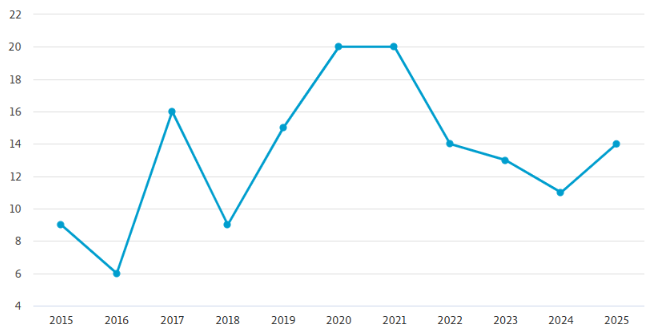
\includegraphics[width=0.9\textwidth]{grafico01-artigos-ano}
  \caption{Distribuição de artigos por ano}
  \fonte{Scopus (2025).}
  \label{graf:ano}
\end{figure}

O Gráfico~\ref{graf:pais} apresenta a distribuição de artigos por país, cujo país com maior quantidade de publicações é os Estados Unidos.

\begin{figure}[H]
  \centering
  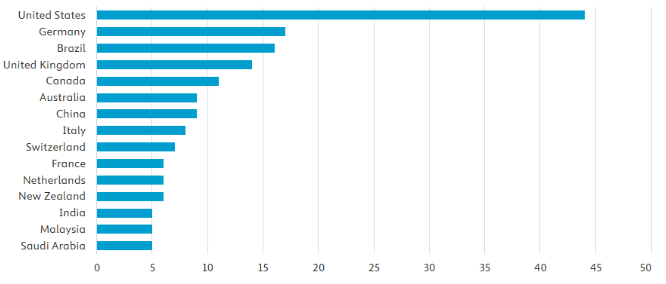
\includegraphics[width=0.9\textwidth]{grafico02-artigos-pais}
  \caption{Distribuição de artigos por país}
  \fonte{Scopus (2025).}
  \label{graf:pais}
\end{figure}

Após a seleção, os materiais foram organizados por categorias temáticas e analisados com base em sua contribuição para a construção do referencial teórico e para o delineamento metodológico da pesquisa. Desse modo, foi utilizada a estratégia da análise de títulos e resumos dos artigos selecionados, para que os resultados possam ser auditáveis, replicáveis e úteis no suporte a pesquisas relacionadas a sistemas de captação de doadores de sangue, com o fim de que hospitais e hemocentros tenham estoques suficientes para atender às necessidades de pacientes que precisam de transfusões sanguíneas em diversas situações.

Sendo assim, a lista de artigos selecionados é apresentada no Quadro~\ref{tab:artigos}.

\begin{table}[H]
  \centering
  \caption{Lista de artigos selecionados}
  \label{tab:artigos}
  \begin{tabularx}{\textwidth}{>{\raggedright\arraybackslash}X >{\raggedright\arraybackslash}p{5.2cm}}
    \toprule
    \textbf{Título} & \textbf{Fonte} \\
    \midrule
    Blood donation support application: Contributions from experts on the tool's functionality
    & Da Silva; Praça Brasil; De Vasconcelos Filho; Brasil; Paiva; De Oliveira; Dos Santos (2021) \\
    \addlinespace
    Effective methods for reactivating inactive blood donors: A stratified randomised controlled study
    & Ou-Yang; Bei; Liang; He; Chen; Fu (2020) \\
    \addlinespace
    Evaluation of the Wateen App in the Blood-Donation Process in Saudi Arabia
    & Alessa (2022) \\
    \addlinespace
    Mobile applications for encouraging blood donation: A systematic review and case study
    & Li; Valero; Keyser; Ukuku; Zheng (2023) \\
    \bottomrule
  \end{tabularx}
  \fonte{Elaborado pelos próprios autores (2025).}
\end{table}

\section{Resultados e discussões}

A análise dos artigos selecionados permitiu identificar um conjunto relevante de soluções tecnológicas voltadas para a captação, o incentivo e a retenção de doadores de sangue, respondendo diretamente aos questionamentos levantados no protocolo de pesquisa. O levantamento revelou uma predominância de aplicativos móveis dedicados a facilitar a interação entre a população e os centros de saúde. Entre as plataformas destacadas na literatura, evidencia-se o Do-eSangue, desenvolvido com o intuito de apoiar a captação e fidelização ao integrar-se diretamente com a base de dados dos hemocentros, permitindo agendamentos e o acesso a informações personalizadas \citeonline{dasilva2021}. No cenário internacional, o Wateen, iniciativa do Ministério da Saúde da Arábia Saudita, atua de forma semelhante no recrutamento e agendamento via dispositivos móveis \citeonline{alessa2022}. Outras iniciativas relevantes incluem o Blood Hero, que explora técnicas de incentivo social para alavancar os estoques \citeonline{li2023}, e o Blood Note, focado em promover a doação por meio de testes preliminares de elegibilidade realizados diretamente pelo celular do usuário \citeonline{li2023}.

No que tange à aplicação de algoritmos de recomendação ou mecanismos inteligentes de sugestão de ações, os estudos apontam para o uso de filtros dinâmicos e cruzamento de dados como alternativas eficientes de conexão. O aplicativo Do-eSangue, por exemplo, realiza o disparo de convites segmentados com base no tipo sanguíneo, na localização geográfica e na necessidade de fenótipos raros. Embora o estudo não utilize a nomenclatura estrita de ``algoritmos de recomendação'', essa filtragem avançada e baseada em critérios específicos de demanda atua, na prática, como uma recomendação direcionada de doadores \citeonline{dasilva2021}. Paralelamente, o Wateen demonstra um mecanismo ágil de correspondência ao notificar usuários específicos quando há demanda hospitalar por sua tipagem sanguínea, permitindo ainda que o próprio doador compartilhe a solicitação com sua rede de contatos, criando um fluxo orgânico e eficiente de recomendações \citeonline{alessa2022}.

Além da infraestrutura técnica de conexão, os trabalhos mapeados evidenciam diversas funcionalidades e estratégias de incentivo essenciais para a promoção contínua da doação. A comunicação personalizada e direcionada surge como um fator crítico nesse cenário. \citeonline{ouyang2020} demonstraram que, para reativar doadores inativos, o contato direto via chamadas telefônicas apresenta resultados significativamente superiores ao uso de SMS, pois viabiliza um diálogo individualizado capaz de resolver barreiras pessoais e motivar o retorno. Aliado a isso, o uso estratégico de redes sociais e a disponibilização de informações abrangentes integradas aos sistemas ajudam a combater mitos, esclarecer dúvidas frequentes e detalhar os critérios de elegibilidade, aumentando a confiança da população nos serviços de saúde.

Outro ponto de forte convergência entre as pesquisas é a adoção da gamificação e de recursos de fidelização. A implementação de sistemas de pontuação, medalhas virtuais (\textit{badges}) e programas de fidelidade que garantem preferência no atendimento servem como um forte apelo de reconhecimento social do voluntário, incentivando a repetição do ato solidário \citeonline{li2023}.

Por fim, a literatura destaca que a otimização da experiência prática do doador é indispensável. Funcionalidades como o agendamento simplificado reduzem drasticamente o tempo de espera e as filas nos hemocentros, fatores que impactam diretamente na satisfação geral do usuário \citeonline{alessa2022}. Quando essas plataformas permitem que o voluntário acompanhe seu histórico de doações e acesse laudos de exames de forma unificada, consolida-se um sentimento de propósito e cuidado com a própria saúde, evidenciando o potencial da tecnologia como ferramenta de transformação na hemoterapia.

\section{Considerações}

O mapeamento sistemático da literatura apresentado neste capítulo permitiu traçar um panorama claro sobre o uso da tecnologia como aliada na captação e retenção de doadores de sangue. Os resultados evidenciam que a adoção de sistemas computacionais --- especialmente aplicativos móveis --- deixou de ser uma inovação distante para se tornar uma necessidade estratégica na gestão hemoterápica. Funcionalidades como o envio de notificações segmentadas, o agendamento prévio e a aplicação de técnicas de gamificação provaram ser eficazes para engajar a população e reduzir os índices de desabastecimento nos estoques.

Apesar das contribuições valiosas encontradas na literatura, nota-se que grande parte dos estudos concentra sua análise nas interfaces com o usuário final e nas estratégias de marketing social, abordando de forma superficial a engenharia de software e a arquitetura estrutural que sustentam essas soluções. Existe uma lacuna no detalhamento de como as complexas regras de negócio desse domínio --- que envolvem critérios médicos de elegibilidade, tipagem sanguínea e urgência hospitalar --- são modeladas e processadas nos bastidores das aplicações.

Nesse sentido, os achados desta revisão validam a proposta central deste Trabalho de Conclusão de Curso. Ao constatar que a filtragem e a recomendação direcionada são os motores do sucesso das ferramentas atuais, reforça-se a relevância de uma API RESTful especializada, estruturada sobre DDD e princípios SOLID conforme discutido no Capítulo~2. O Capítulo~5 apresenta o estudo de caso, detalhando como os requisitos, a modelagem do domínio e a implementação da solução tratam, na prática, as lacunas de engenharia de software identificadas nesta revisão.

\chapter{Métodos e recursos}

Neste capítulo são descritos os procedimentos metodológicos adotados para o alcance dos objetivos propostos, abordando a abordagem de pesquisa escolhida, os instrumentos utilizados na coleta e análise de informações e as ferramentas empregadas no desenvolvimento da API.

\section{Visão geral}

Para o desenvolvimento da pesquisa adotou-se a abordagem qualitativa, que se destaca por enfatizar a análise de dados não numéricos, como documentos, normativas e literatura especializada, buscando compreender o significado e a complexidade dos fenômenos investigados.

\begin{citacao}
A pesquisa qualitativa trabalha com o universo de significados, motivos, aspirações, crenças, valores e atitudes, o que corresponde a um espaço mais profundo das relações, dos processos e dos fenômenos que não pode ser reduzido à operacionalização de variáveis. \cite[p.~21]{minayo2001}
\end{citacao}

Para a condução do trabalho, foram traçadas etapas sequenciais, ilustradas na Figura~\ref{fig:processo-tcc} e na Figura~\ref{fig:processo-api}.

\begin{figure}[H]
  \centering
  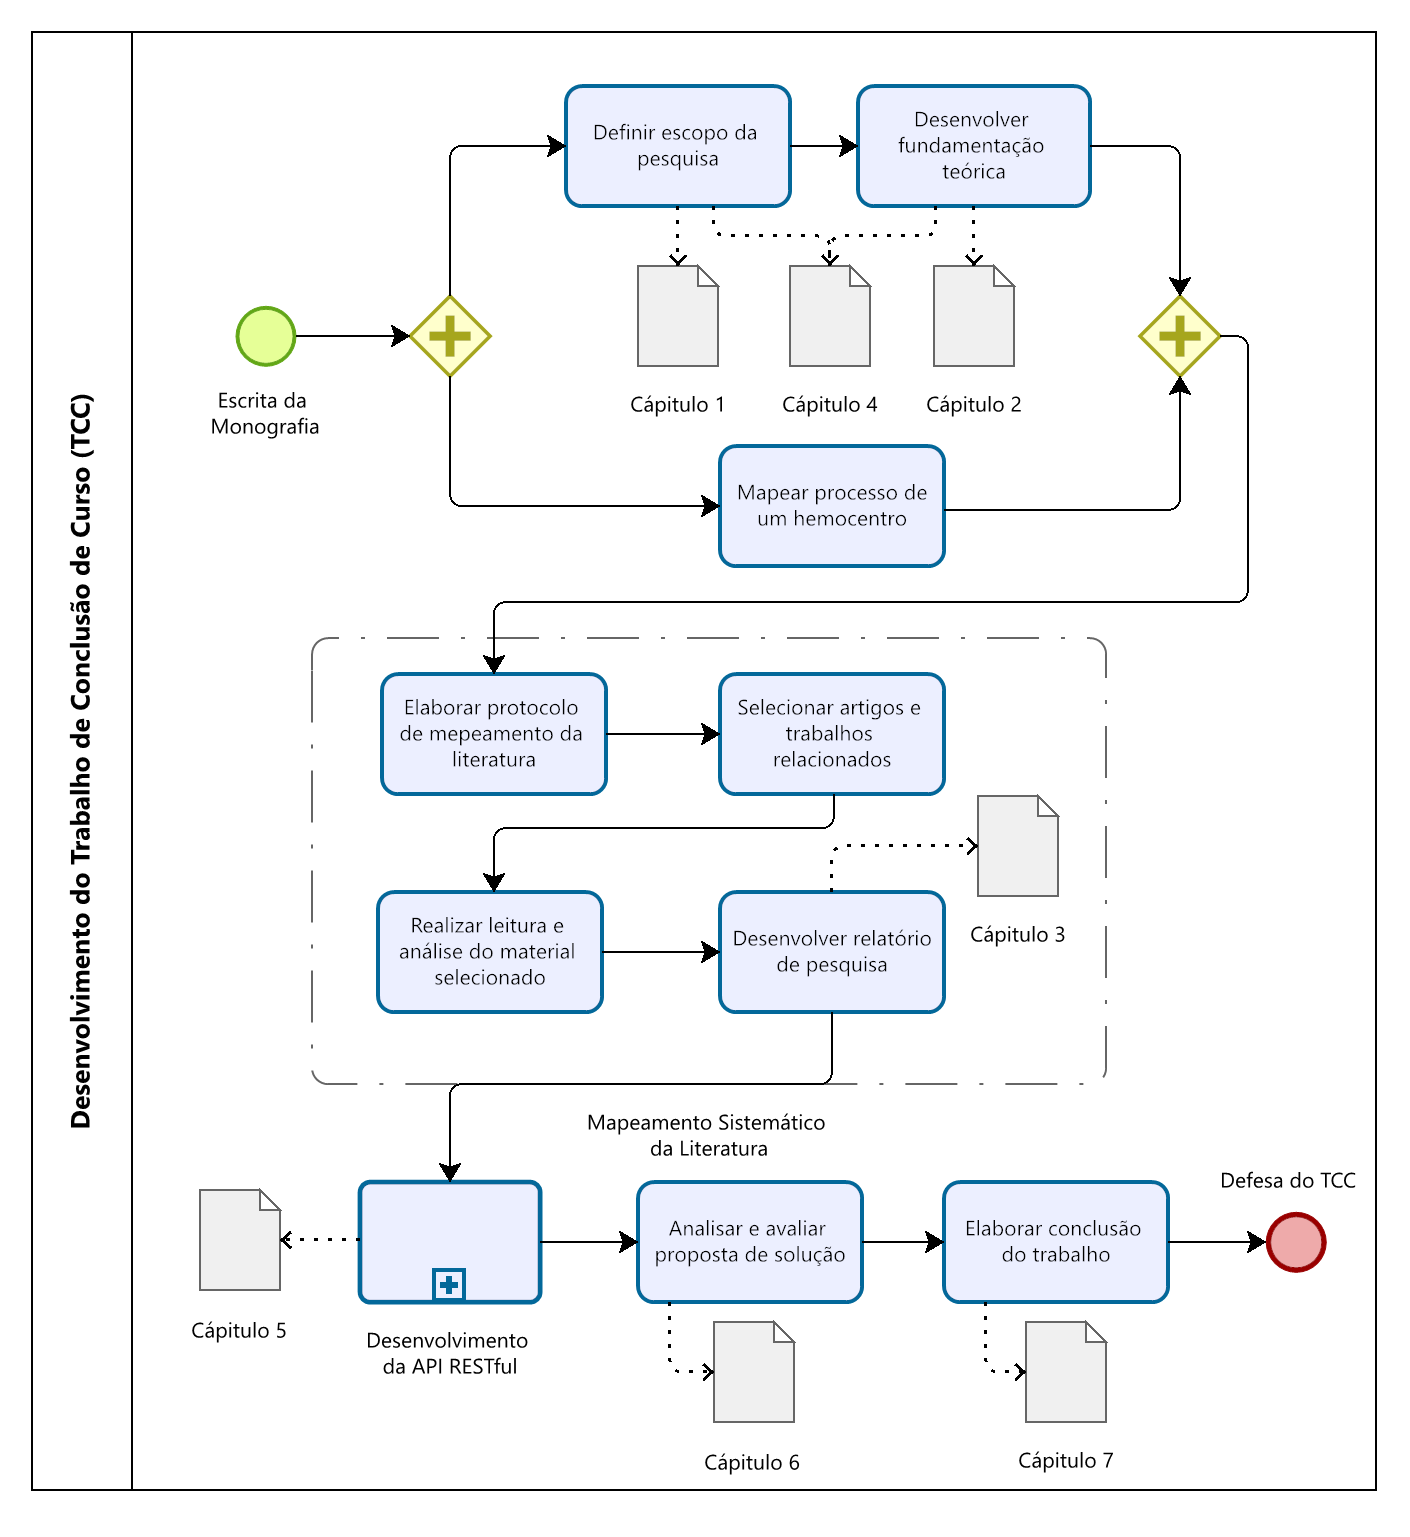
\includegraphics[width=0.95\textwidth]{figura01-processo-tcc}
  \caption{Diagrama de processos do desenvolvimento do TCC}
  \fonte{Elaborado pelos próprios autores (2025).}
  \label{fig:processo-tcc}
\end{figure}

\begin{figure}[H]
  \centering
  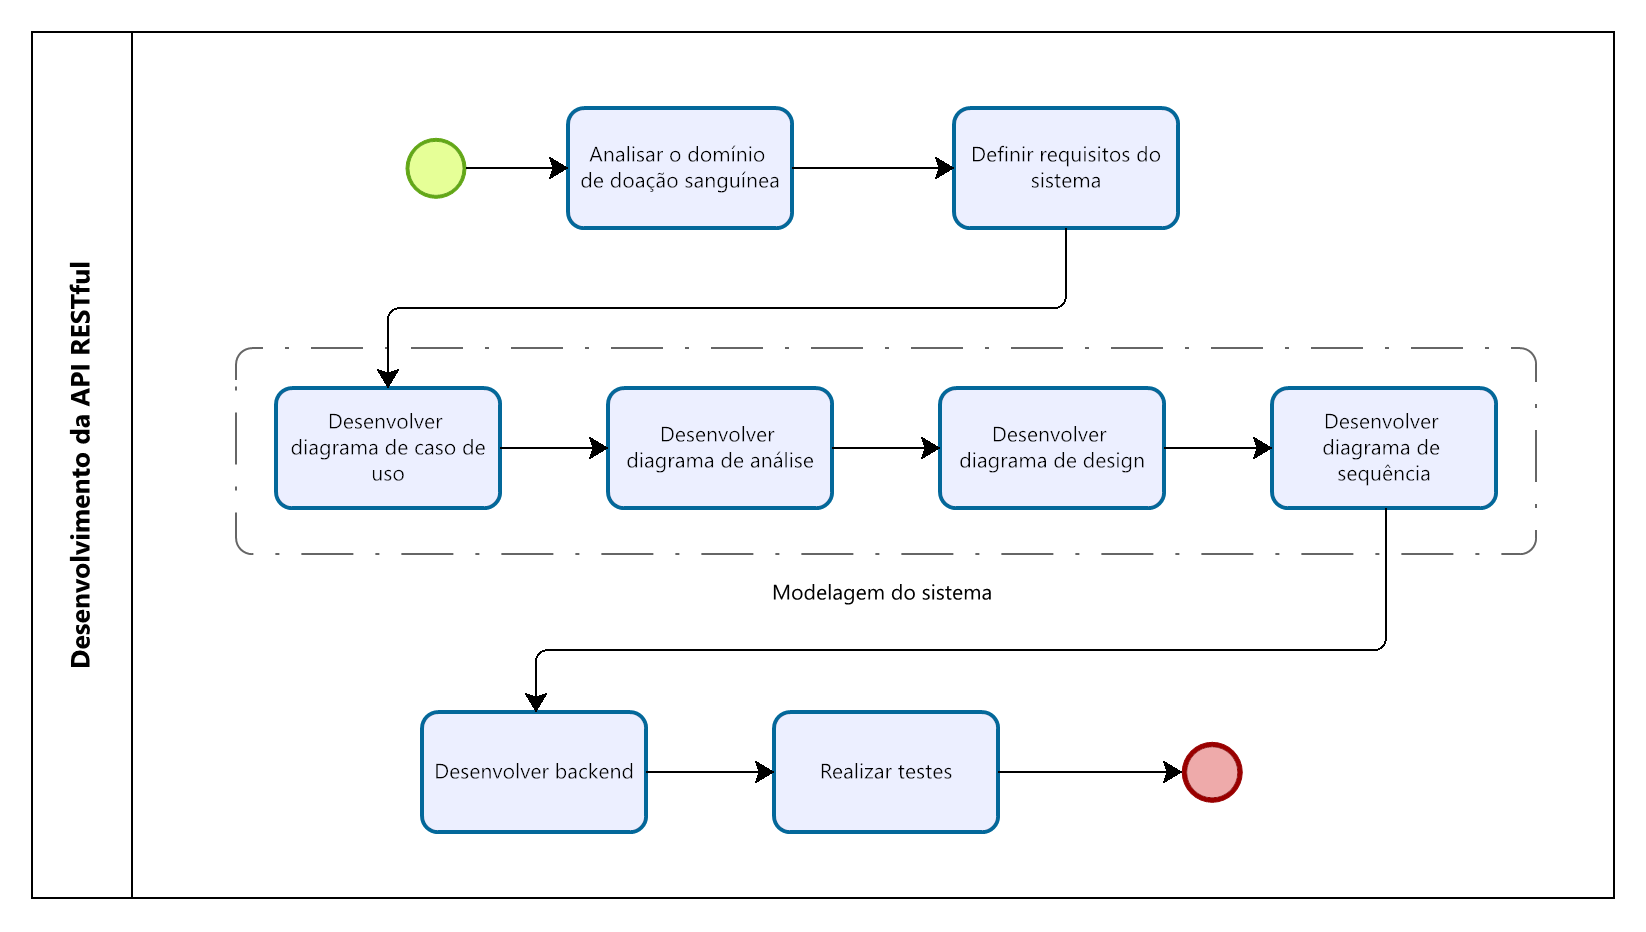
\includegraphics[width=0.95\textwidth]{figura02-processo-api}
  \caption{Diagrama de processos do Desenvolvimento da API}
  \fonte{Elaborado pelos próprios autores (2025).}
  \label{fig:processo-api}
\end{figure}

Inicialmente, definiu-se o escopo da pesquisa, o problema, as justificativas e os objetivos que fundamentam o Capítulo~1. Em seguida, conduziu-se o levantamento bibliográfico sobre OO, SOLID e DDD, aprofundados no Capítulo~2.

Paralelamente, realizou-se o mapeamento do processo de um hemocentro por meio de pesquisa documental e bibliográfica, buscando compreender o fluxo de trabalho, as regras de negócio e as necessidades do domínio da doação de sangue. Elaborou-se também um protocolo de mapeamento sistemático da literatura, cujos resultados são discutidos no Capítulo~3.

Com base no conhecimento adquirido nessas etapas, realizou-se a análise do domínio sob a ótica do DDD e a definição dos requisitos funcionais e não funcionais. Na sequência, elaborou-se o projeto da solução (casos de uso e diagramas de classes) e desenvolveu-se a API aplicando SOLID, com vistas à escalabilidade, manutenibilidade e testabilidade.

Por fim, os resultados foram avaliados por meio de testes unitários e de integração, seguidos da elaboração das conclusões do trabalho.

\section{Instrumentos e ferramentas}

Para a coleta e análise dos dados, foram utilizados instrumentos compatíveis com os objetivos e a abordagem metodológica da pesquisa, orientados pela necessidade de obter informações confiáveis e contextualizadas sobre o cenário da doação de sangue e sobre as tecnologias empregadas no desenvolvimento da API.

\subsection{Pesquisa exploratória-descritiva}

A presente pesquisa caracteriza-se como exploratória-descritiva, abordagem que, segundo \citeonline{gil2008}, proporciona maior familiaridade com o problema investigado e, simultaneamente, descreve as características do fenômeno estudado. Segundo \citeonline{prodanov2013}, essa combinação metodológica é especialmente adequada para estudos que envolvem questões sociais e de saúde pública, permitindo uma análise contextualizada e orientada para a intervenção.

O contexto de análise adotado foi o das normativas e do cenário de atuação dos hemocentros, com atenção às demandas da região de Campos dos Goytacazes, local de moradia e estudo dos pesquisadores. Essa escolha favoreceu maior familiaridade com os aspectos sociais, culturais e institucionais que envolvem a temática, além de facilitar o acesso a dados públicos e normativas das unidades hospitalares e hemocentros locais.

Segundo \citeonline{pressman2016}, o esforço inicial de compreensão do domínio e das necessidades reais dos \textit{stakeholders} é indispensável para criar uma base sólida de requisitos e evitar o desenvolvimento de sistemas inadequados à realidade operacional. Nesse sentido, utilizou-se a análise documental e bibliográfica como técnica de coleta de dados, por permitir profundidade na obtenção de informações normativas e procedimentais a partir de manuais do Ministério da Saúde, portarias vigentes e literatura acadêmica.

Segundo \citeonline{marconi2003}, a pesquisa documental é composta por etapas fundamentais --- como a seleção, leitura crítica e categorização dos dados --- que garantem a sistematização e a confiabilidade das informações obtidas. \citeonline{sommerville2011} reforça que a análise de documentos atua como instrumento de captura e construção do conhecimento, sendo essencial para a engenharia de requisitos em sistemas críticos, como os voltados à saúde pública.

O levantamento realizado a partir de documentos oficiais e estudos de caso sobre triagem, captação e gestão em hemocentros teve como objetivo compreender os fatores que influenciam a decisão de doar sangue, identificar barreiras e motivações entre potenciais doadores descritos na literatura, e subsidiar os requisitos da API proposta.

\subsection{Desenvolvimento da API}

O desenvolvimento da API foi orientado por boas práticas de engenharia de \textit{software}, com foco na escalabilidade, na manutenibilidade e na clareza estrutural do código. Adotou-se DDD e SOLID como diretrizes arquiteturais (Seções~\ref{sec:ddd} e~\ref{sec:solid}). A camada de segurança contempla autenticação baseada em \textit{JSON Web Token} (JWT), padrão amplamente adotado em APIs RESTful para autenticação sem estado (\textit{stateless}).

\subsubsection{Linguagem de programação (Java)}

A linguagem escolhida para a implementação foi o Java, em sua versão 17 (\textit{Long Term Support} --- LTS). Java é uma linguagem orientada a objetos, fortemente tipada e amplamente documentada na literatura \cite{deitel2017}. A tipagem estática do Java favorece a implementação de \textit{Value Objects} e \textit{Entities}, garantindo que erros de domínio sejam capturados em tempo de compilação. Em contrapartida, uma crítica comum ao Java é a sua verbosidade e o consumo de memória da \textit{Java Virtual Machine} (JVM), se comparado a linguagens como Go ou Python, conforme discutido por \citeonline{bloch2018}. Ainda assim, a robustez da linguagem compensa essas restrições para o contexto corporativo.

\subsubsection{\textit{Framework} de desenvolvimento (Spring Boot)}

Para agilizar o desenvolvimento e a configuração da infraestrutura, utilizou-se o \textit{framework} Spring Boot. Segundo \citeonline{walls2019}, o Spring Boot aplica o conceito de ``convenção sobre configuração'', permitindo que o desenvolvedor foque na lógica de negócio enquanto o \textit{framework} gerencia a injeção de dependência e a conexão com o banco de dados. Por outro lado, a facilidade do Spring pode esconder a complexidade subjacente, dificultando o \textit{debug} (depuração) caso o desenvolvedor não entenda o ciclo de vida dos \textit{beans} gerenciados pelo \textit{container}.

\subsubsection{Ambiente de desenvolvimento e versionamento (Visual Studio Code e Git)}

Para a codificação, utilizou-se o editor de código Visual Studio Code (VS Code), devido ao seu vasto ecossistema de extensões para Java e suporte nativo a terminais leves. Para o controle de versão, adotou-se o Git, hospedando o repositório na plataforma GitHub. Segundo \citeonline{chacon2014}, o versionamento distribuído é essencial para manter o histórico de alterações seguro e permitir ramificações (\textit{branches}) para testes de novas funcionalidades sem comprometer o código estável (\textit{main}).
\chapter{API RESTful proposta: requisitos, análise, design e implementação}

\section{Visão geral da solução}

Este capítulo apresenta a solução tecnológica desenvolvida para apoiar o processo de captação e gerenciamento de solicitações de doação de sangue. A proposta materializa-se na construção de uma API RESTful focada exclusivamente na camada de \textit{backend}, responsável pelo gerenciamento de participantes (pessoas e organizações), solicitações de doação, registro do histórico de doadores e recomendação de solicitações compatíveis.

O desenvolvimento foi orientado pelos princípios do DDD e pelos princípios SOLID, já fundamentados no Capítulo~2. Essa abordagem permitiu que a estrutura do software refletisse a realidade do domínio da hemoterapia, reduzindo o acoplamento entre os componentes e facilitando a evolução contínua do sistema. As seções seguintes detalham o levantamento de requisitos, a modelagem do sistema, a organização do domínio e da arquitetura, a implementação técnica e, por fim, a estratégia de recomendação e de cumprimento de metas, que constitui o núcleo funcional da API.

\section{Levantamento de requisitos}

A extração de requisitos ocorreu a partir da análise documental e bibliográfica descrita no Capítulo~4, alinhando as necessidades dos diferentes atores envolvidos no processo de doação de sangue às capacidades técnicas do sistema proposto.

Os requisitos funcionais representam as operações que a API disponibiliza para atender às rotinas de cadastro, gerenciamento de solicitações, recomendação e controle de doações. A tabela~\ref{tab:rf} sintetiza as funcionalidades identificadas e implementadas, refletindo diretamente os recursos (\textit{endpoints}) expostos pela API.

\begin{table}[H]
  \centering
  \caption{Requisitos funcionais}
  \label{tab:rf}
  \small
  \begin{tabularx}{\textwidth}{c X}
    \toprule
    \textbf{Código} & \textbf{Descrição} \\
    \midrule
    RF01 & Permitir o cadastro de pessoas no sistema. \\
    RF02 & Permitir o cadastro de organizações no sistema. \\
    RF03 & Permitir que uma pessoa cadastrada registre um perfil de doador. \\
    RF04 & Permitir que uma pessoa ou organização registre um perfil de requisitante. \\
    RF05 & Permitir que uma organização cadastrada registre um perfil de banco de sangue (hemocentro). \\
    RF06 & Permitir a autenticação de usuários por meio de credenciais válidas, emitindo um JWT. \\
    RF07 & Permitir a atualização dos dados cadastrais de um participante (\textit{party}). \\
    RF08 & Permitir a atualização do perfil e das preferências de recomendação do doador. \\
    RF09 & Permitir que requisitantes criem solicitações de doação de sangue. \\
    RF10 & Permitir a atualização dos dados de uma solicitação (meta de bolsas e/ou data-limite). \\
    RF11 & Permitir o cancelamento de uma solicitação de doação. \\
    RF12 & Permitir a consulta das solicitações de doação de um participante. \\
    RF13 & Permitir a consulta das solicitações de doação recomendadas para um doador. \\
    RF14 & Permitir a notificação de doadores potenciais elegíveis para uma solicitação. \\
    RF15 & Permitir o registro de uma doação, informando a data de intenção (pendente) ou a data efetiva (concluída). \\
    RF16 & Permitir o reagendamento de uma doação pendente. \\
    RF17 & Permitir a confirmação (conclusão) de uma doação pendente. \\
    RF18 & Permitir a consulta do histórico de doações de um doador. \\
    RF19 & Permitir a consulta do resumo (\textit{summary}) de um doador. \\
    \bottomrule
  \end{tabularx}
  \fonte{Elaborado pelos próprios autores (2026).}
\end{table}


Ressalta-se que a lista de requisitos funcionais apresentada não tem a pretensão de esgotar todas as rotinas administrativas de um hemocentro ou unidade hospitalar, mas de delimitar um conjunto mínimo e coeso de operações indispensáveis para validar os conceitos teóricos e arquiteturais propostos. Esse escopo abrange o ciclo fundamental da doação de sangue ao contemplar, de maneira integrada, a gestão da demanda (abertura e acompanhamento de solicitações por unidades de saúde e pacientes), a oferta (disponibilidade, elegibilidade e intenções de doação pelos voluntários) e o registro histórico das doações realizadas.


Além das funcionalidades diretas, foram definidos requisitos não funcionais para estabelecer os parâmetros de qualidade, segurança e arquitetura esperados. Considerando a adoção do DDD e da arquitetura em camadas, a Tabela~\ref{tab:rnf} apresenta as diretrizes técnicas estabelecidas para a solução.

\begin{table}[H]
  \centering
  \caption{Requisitos não funcionais}
  \label{tab:rnf}
  \small
  \begin{tabularx}{\textwidth}{c X}
    \toprule
    \textbf{Código} & \textbf{Descrição} \\
    \midrule
    RNF01 & O sistema deve disponibilizar seus serviços por meio de uma API RESTful utilizando o protocolo HTTP. \\
    RNF02 & O sistema deve autenticar usuários por meio de JWT. \\
    RNF03 & O sistema deve persistir os dados em banco de dados NoSQL (MongoDB). \\
    RNF04 & O sistema deve permitir evolução e manutenção sem impacto significativo nas demais camadas da aplicação. \\
    RNF05 & O sistema deve seguir uma arquitetura em camadas orientada pelos princípios do DDD. \\
    RNF06 & O sistema deve aplicar os princípios SOLID para favorecer baixo acoplamento e alta coesão. \\
    RNF07 & A API deve retornar respostas em formato JSON. \\
    RNF08 & O sistema deve validar os dados recebidos antes do processamento das operações. \\
    RNF09 & O sistema deve controlar o acesso às funcionalidades protegidas por meio de autorização baseada em perfis (\textit{roles}) de usuário. \\
    RNF10 & O sistema deve preservar a consistência de escritas concorrentes sobre uma mesma solicitação de doação, evitando a perda de atualizações. \\
    \bottomrule
  \end{tabularx}
  \fonte{Elaborado pelos próprios autores (2026).}
\end{table}


Diferentemente dos requisitos funcionais, que especificam os serviços e as ações que o sistema deve executar, os requisitos não funcionais definem as qualidades, restrições e propriedades estruturais do \textit{software}. Nesse sentido, os itens elencados estabelecem parâmetros de segurança (como autenticação sem estado e autorização por papéis), manutenibilidade e baixo acoplamento (assegurados pela divisão em camadas orientada ao DDD e ao SOLID), integridade de dados (por meio do controle de concorrência otimista) e padronização das comunicações (via API RESTful e formato JSON), sustentando a robustez técnica da solução desenvolvida.


\section{Modelagem do sistema}

Após a consolidação dos requisitos, procedeu-se com a modelagem do sistema para descrever as interações entre os atores e a API, permitindo visualizar o comportamento esperado da solução sob a perspectiva estrutural e de uso.

\subsection{Casos de uso}

A modelagem de casos de uso, em notação UML, sintetiza as operações disponíveis para os diferentes perfis de acesso. A Tabela~\ref{tab:uc} apresenta o mapeamento dos casos de uso e seus respectivos atores, incluindo tanto as operações representadas nos diagramas a seguir quanto operações complementares oferecidas pela API para os mesmos atores.

\begin{table}[H]
  \centering
  \caption{Lista de casos de uso}
  \label{tab:uc}
  \small
  \begin{tabularx}{\textwidth}{c >{\raggedright\arraybackslash}X >{\raggedright\arraybackslash}p{3.2cm}}
    \toprule
    \textbf{Código} & \textbf{Caso de uso} & \textbf{Ator principal} \\
    \midrule
    UC01 & Cadastrar-se como pessoa (\textit{Sign Up as Person}) & Guest \\
    UC02 & Cadastrar-se como organização (\textit{Sign Up as Organization}) & Guest \\
    UC03 & Autenticar (\textit{Authenticate}) & Guest \\
    UC04 & Registrar perfil de doador & Person \\
    UC05 & Registrar perfil de requisitante & Person / Organization \\
    UC06 & Registrar perfil de banco de sangue & Organization \\
    UC07 & Atualizar dados cadastrais (\textit{Update Party}) & Person / Organization \\
    UC08 & Atualizar perfil e preferências do doador (\textit{Update Donor}) & Donor \\
    UC09 & Registrar solicitação de doação (\textit{Register Donation Request}) & Requester \\
    UC10 & Consultar recomendações de solicitações (\textit{Consult Recommendations}) & Donor \\
    UC11 & Registrar doação (\textit{Register Donation}) & Donor \\
    UC12 & Completar doação pendente (\textit{Complete a Pending Donation}) & Donor \\
    UC13 & Consultar histórico de doações (\textit{See Donation History}) & Donor \\
    UC14 & Gerenciar solicitações --- atualizar dados, cancelar e consultar & Requester \\
    UC15 & Notificar doadores potenciais elegíveis & Requester \\
    UC16 & Reagendar doação pendente & Donor \\
    UC17 & Consultar resumo do doador (\textit{Donor Summary}) & Donor \\
    \bottomrule
  \end{tabularx}
  \fonte{Elaborado pelos próprios autores (2026).}
\end{table}

A representação gráfica dessas interações é dividida de acordo com o nível de acesso dos atores. A Figura~\ref{fig:uc-access-baseProfiles} apresenta o diagrama de caso de uso de acesso e perfis base (\textit{Guest, Person and Organization}).

\begin{figure}[H]
  \centering
  \caption{Diagrama de caso de uso de acesso e perfis base}
  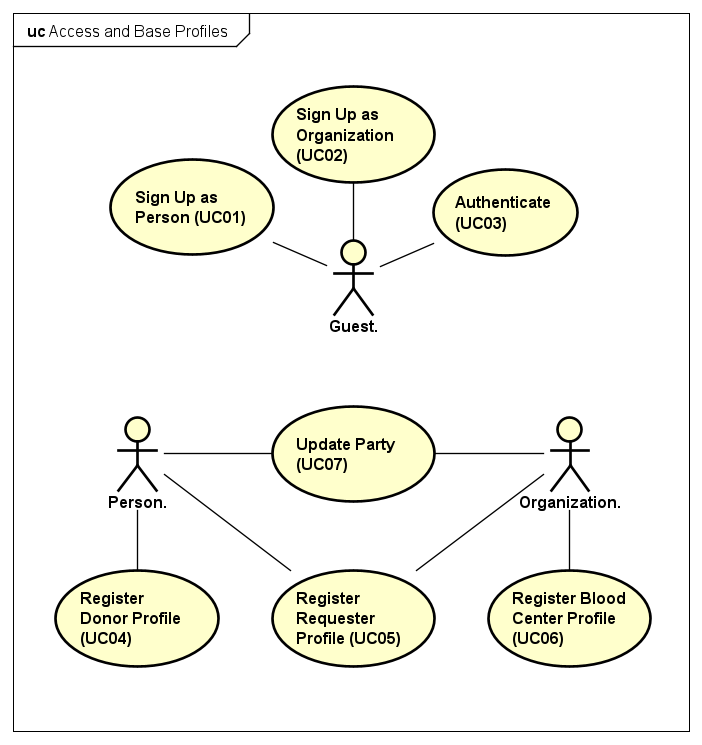
\includegraphics[width=0.6\textwidth]{figura03-uc-acesso-perfisBase}
  \fonte{Elaborado pelos próprios autores (2026).}
  \label{fig:uc-access-baseProfiles}
\end{figure}

O ator \textit{Guest} representa utilizadores sem cadastro prévio, limitados às operações de criação de contas e autenticação (UC01, UC02 e UC03). Os atores \textit{Person} e \textit{Organization} representam os usuários recém-cadastrados, permitindo a atualização de dados da conta (UC07) e a definição de seus papéis específicos no sistema de domínio, como Doador (UC04), Requisitante (UC05) ou Banco de Sangue (UC06).

Já a Figura~\ref{fig:uc-requester} representa o diagrama de caso de uso do ator (\textit{Requester}).

\begin{figure}[H]
  \centering
  \caption{Diagrama de caso de uso de requisitante}
  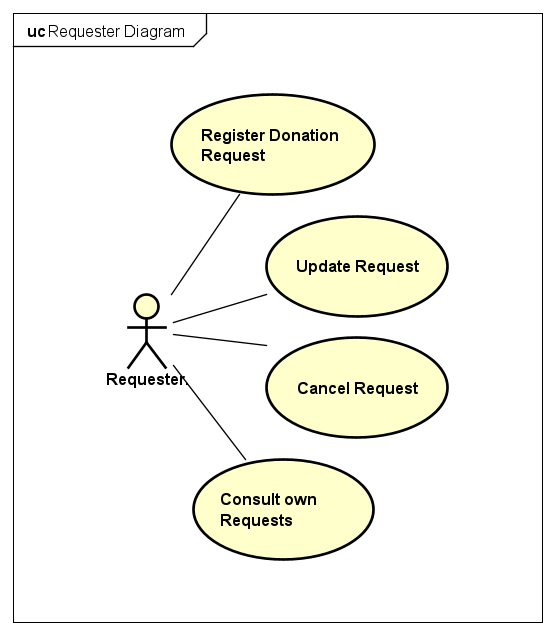
\includegraphics[width=0.65\textwidth]{figura04-uc-requisitante}
  \fonte{Elaborado pelos próprios autores (2026).}
  \label{fig:uc-requester}
\end{figure}

O ator \textit{Requester} concentra as permissões relacionadas à criação de solicitações de doação (UC09) e à sua gestão (UC14), além do disparo de notificações a doadores potenciais quando uma solicitação necessita de maior alcance (UC15).

Por fim, a Figura~\ref{fig:uc-donor} representa o diagrama de caso de uso do ator (\textit{Donor}).

\begin{figure}[H]
  \centering
  \caption{Diagrama de caso de uso de doador}
  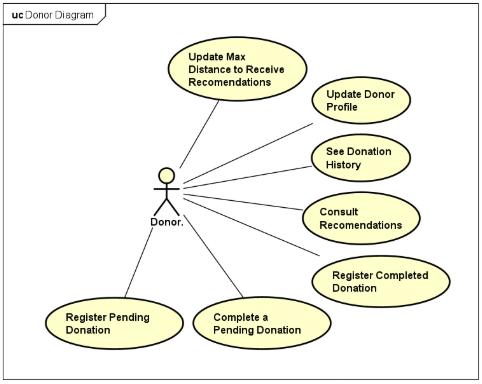
\includegraphics[width=0.7\textwidth]{figura05-uc-doador}
  \fonte{Elaborado pelos próprios autores (2026).}
  \label{fig:uc-donor}
\end{figure}

O ator \textit{Donor} possui acesso ao núcleo do processo de doação, incluindo a atualização de seu perfil clínico (UC08), a consulta às solicitações recomendadas (UC10), o registro unificado de doações (UC11), a conclusão (UC12) e o reagendamento de doações pendentes (UC16), a consulta ao próprio histórico hemoterápico (UC13) e a emissão de seu resumo (UC17). Vale ressaltar que, no UC11, a doação nasce pendente quando o doador informa a data de intenção ou concluída quando informa a data efetiva --- um único caso de uso, sem fábricas concorrentes no domínio.

\subsubsubsection{Detalhamento dos casos de uso}

Devido à abrangência da API e visando manter a concisão documental, optou-se por detalhar apenas os casos de uso críticos para o núcleo da aplicação, adotando a estrutura formal de especificação textual proposta por Cockburn (2001). Essa abordagem documenta o fluxo de eventos, as restrições operacionais e as pré-condições de segurança exigidas, justificando arquiteturalmente a ausência de relacionamentos visuais de dependência de autenticação nos diagramas UML. A Tabela~\ref{tab:detalhamento-uc} sintetiza essas especificações.

\begin{table}[H]
  \centering
  \caption{Especificação dos casos de uso críticos}
  \label{tab:detalhamento-uc}
  \small
  \begin{tabularx}{\textwidth}{>{\bfseries}p{3.3cm} X}
    \toprule
    \multicolumn{2}{l}{\textbf{UC09: Registrar solicitação de doação}} \\
    \midrule
    Ator principal & Requisitante (\textit{Requester}) \\
    Pré-condição & Usuário autenticado com perfil de Requisitante ativo. \\
    Fluxo principal & 
    1. O Requisitante solicita a criação de uma nova campanha.\\
    & 2. Informa dados da necessidade (tipo sanguíneo, bolsas, prazo, urgência e hemocentro).\\
    & 3. O sistema valida as regras de negócio e os invariantes de domínio.\\
    & 4. O sistema persiste a solicitação no estado ativo.\\
    & 5. O sistema retorna a confirmação com o identificador único gerado. \\
    Cenário alternativo & \textbf{3a.} Falha de validação (prazo retroativo ou meta nula): rejeita a operação e retorna mensagem de erro estruturada. \\
    \midrule
    \multicolumn{2}{l}{\textbf{UC10: Consultar recomendações de solicitações}} \\
    \midrule
    Ator principal & Doador (\textit{Donor}) \\
    Pré-condição & Usuário autenticado com perfil de Doador ativo. \\
    Fluxo principal & 
    1. O Doador solicita a consulta de campanhas recomendadas.\\
    & 2. O sistema avalia a elegibilidade temporal com base na última doação.\\
    & 3. O sistema recupera solicitações ativas e avalia a compatibilidade tipológica.\\
    & 4. O sistema aplica o filtro geoespacial pela distância máxima configurada.\\
    & 5. O sistema ordena por urgência, proximidade e prazo, retornando a listagem. \\
    Cenário alternativo & \textbf{2a.} Doador temporariamente inelegível: encerra o processamento e retorna listagem vazia. \\
    \midrule
    \multicolumn{2}{l}{\textbf{UC12: Completar doação pendente}} \\
    \midrule
    Ator principal & Doador (\textit{Donor}) \\
    Pré-condição & Usuário autenticado com perfil de Doador ativo. \\
    Fluxo principal & 
    1. O Doador submete a data de efetivação de intenção previamente registrada.\\
    & 2. O sistema recupera a doação pendente associada ao identificador.\\
    & 3. O sistema valida a consistência cronológica em relação à data corrente.\\
    & 4. O sistema transiciona o estado do agregado para concluído.\\
    & 5. O sistema atualiza o registro do doador, recalculando a janela de descanso regulamentar. \\
    Cenário alternativo & \textbf{3a.} Data inconsistente (data futura): rejeita a atualização e mantém a doação pendente. \\
    \bottomrule
  \end{tabularx}
  \fonte{Elaborado pelos próprios autores (2026).}
\end{table}

\subsection{Diagramas de classes}

Para representar a estrutura estática da aplicação e evidenciar a aplicação do DDD na prática --- cujos conceitos de entidade, agregado e objeto de valor já foram apresentados no Capítulo~2 ---, a modelagem de classes foi concebida em duas perspectivas distintas: conceitual e de implementação. A perspectiva conceitual mapeia o vocabulário do negócio e as relações semânticas do mundo real, omitindo métodos e tipos de dados para facilitar a validação com especialistas. Em contrapartida, a perspectiva de implementação atua como uma representação estrutural do código-fonte construído, detalhando os limites transacionais, o encapsulamento e as diretrizes arquiteturais.

A Figura~\ref{fig:classe-participantes} apresenta o diagrama de classes conceitual focado nos participantes e em seus papéis (\textit{Roles}).

\begin{figure}[H]
  \centering
  \caption{Diagrama conceitual dos participantes}
  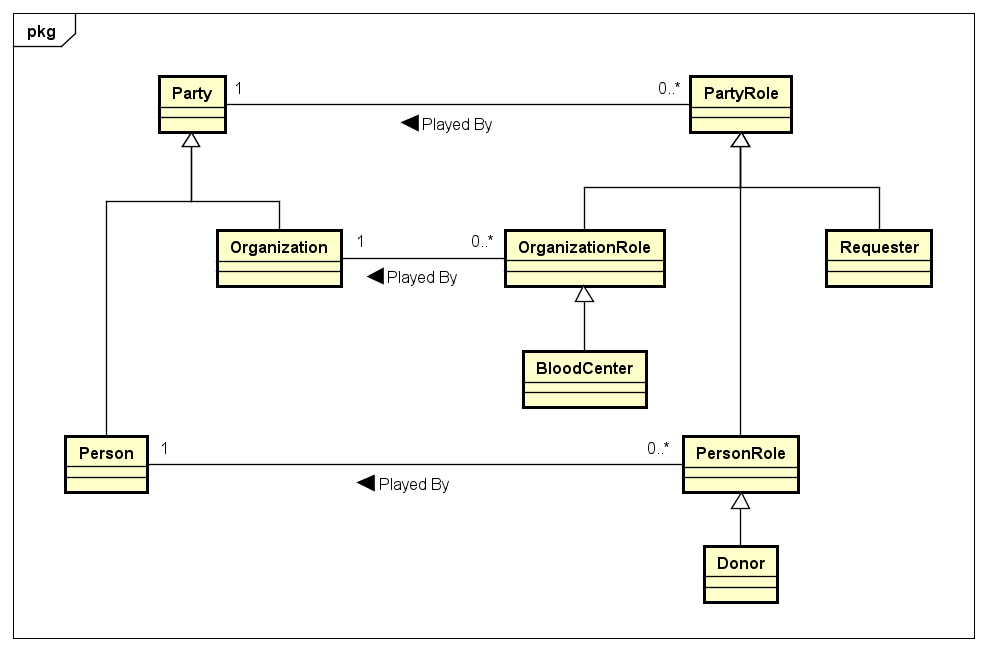
\includegraphics[width=0.65\textwidth]{figura06-classes-participantes}
  \fonte{Elaborado pelos próprios autores (2026).}
  \label{fig:classe-participantes}
\end{figure}

Observa-se a utilização da abstração central \texttt{Party}, que atua como classe base para \texttt{Person} (Pessoa) e \texttt{Organization} (Organização). Essa modelagem reflete a flexibilidade do domínio, permitindo que as entidades assumam múltiplos papéis, como \texttt{Donor} (Doador) e \texttt{Requester} (Requisitante), eliminando a duplicidade de dados no sistema.

Dando prosseguimento à representação do negócio, a Figura~\ref{fig:classe-doacao} ilustra o diagrama de classes conceitual do processo de doação.

\begin{figure}[H]
  \centering
  \caption{Diagrama conceitual do processo de doação}
  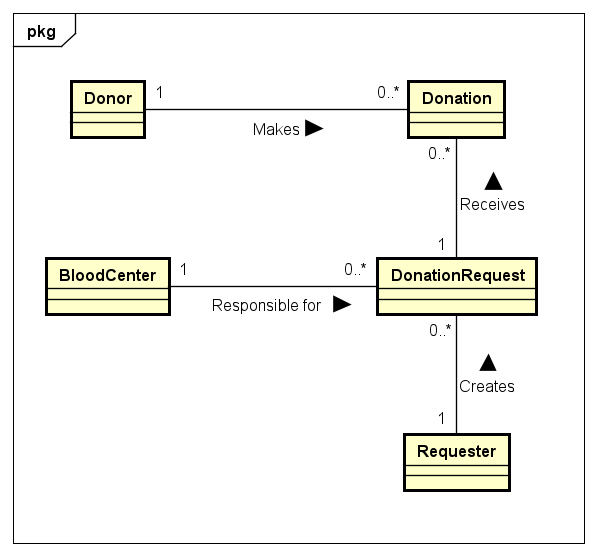
\includegraphics[width=0.65\textwidth]{figura07-classes-doacao}
  \fonte{Elaborado pelos próprios autores (2026).}
  \label{fig:classe-doacao}
\end{figure}

Neste nível de abstração, evidencia-se a associação semântica entre a solicitação (\codigo{DonationRequest}) e o ato de doar (\codigo{Donation}). O fluxo natural demonstra que um \codigo{Requester} origina a solicitação, que é vinculada a um \codigo{BloodCenter} e, posteriormente, recebe as doações efetivadas por um \codigo{Donor}.

Elevando o rigor para o design de software, a Figura~\ref{fig:impl-request} detalha a implementação técnica do agregado \texttt{DonationRequest}.

\begin{figure}[H]
  \centering
  \caption{Diagrama de implementação: agregado DonationRequest}
  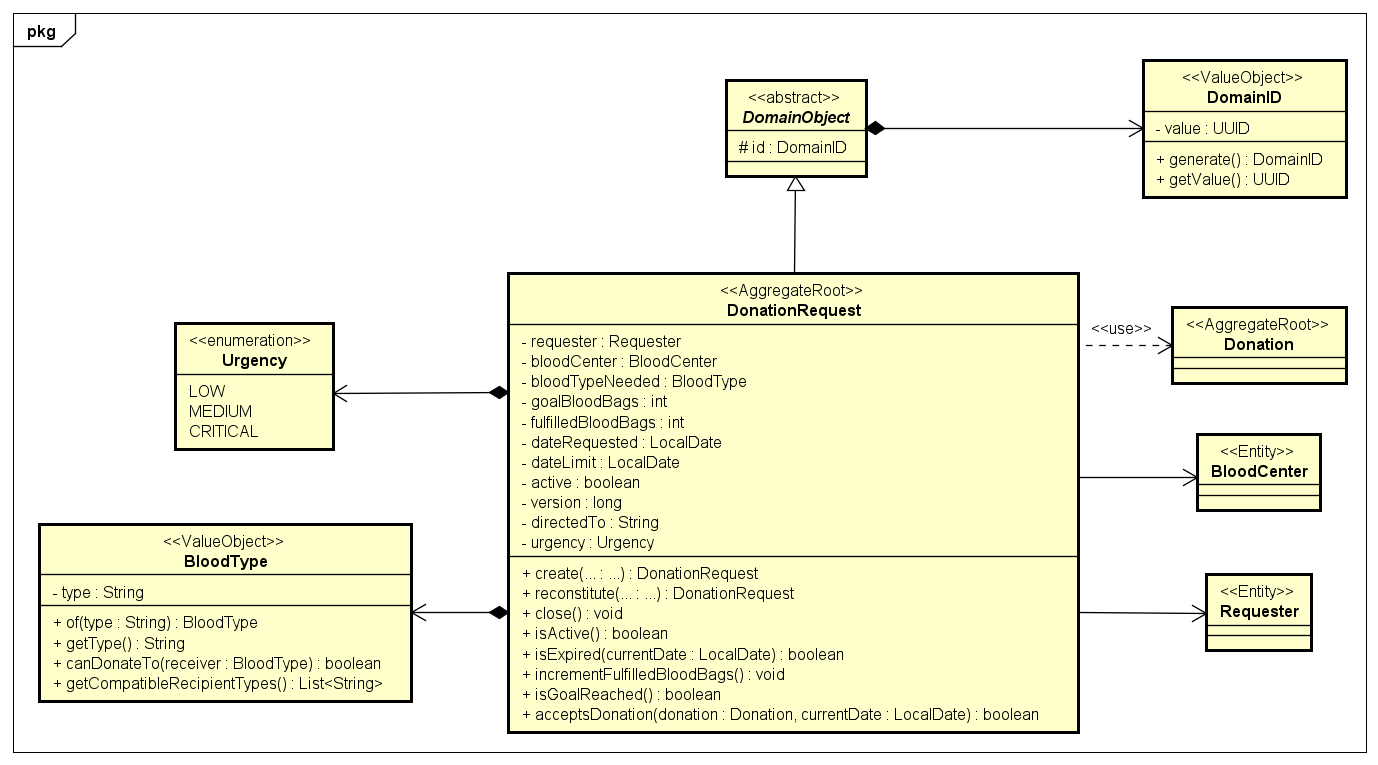
\includegraphics[width=0.9\textwidth]{figura08-impl-donation-request}
  \fonte{Elaborado pelos próprios autores (2026).}
  \label{fig:impl-request}
\end{figure}

A classe é modelada como uma raiz de agregado (\texttt{<<AggregateRoot>>}), atuando como a única porta de entrada para a proteção de invariantes, como as datas-limite e a urgência da solicitação. Observa-se a aplicação da herança por meio da superclasse abstrata \texttt{DomainObject}, responsável por compor os identificadores únicos globais (\texttt{<<ValueObject>> DomainID}). Destaca-se também a dependência tracejada (\texttt{<<use>>}) com a classe \texttt{Donation}, a qual evidencia o baixo acoplamento da arquitetura: a requisição não armazena doações em memória, apenas as avalia de forma transitória por meio de parâmetros no método \texttt{acceptsDonation()}.

Por fim, a Figura~\ref{fig:impl-donation} apresenta o diagrama de implementação do agregado \texttt{Donation}.

\begin{figure}[H]
  \centering
  \caption{Diagrama de implementação: agregado Donation}
  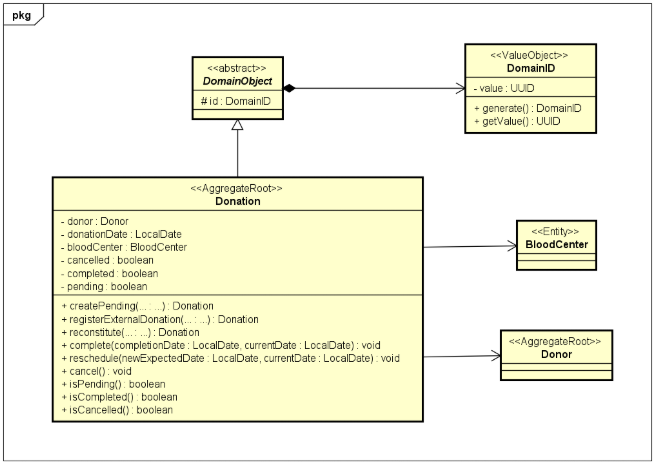
\includegraphics[width=0.75\textwidth]{figura09-impl-donation}
  \fonte{Elaborado pelos próprios autores (2026).}
  \label{fig:impl-donation}
\end{figure}

Tratada também como uma raiz de agregado autônoma, a classe concentra uma única fábrica \codigo{create} e o ciclo de vida pendente--concluída--cancelada. O estado não é armazenado como flags independentes: deriva das datas de intenção (\codigo{intendedDate}), de efetivação (\codigo{donationDate}) e de cancelamento (\codigo{cancelledAt}). Completar uma doação pendente preenche a data efetiva sem apagar a intenção; reagendar e cancelar permanecem transições sobre o mesmo agregado. A navegabilidade unidirecional explícita demonstra que a doação possui a referência imediata do \texttt{Donor} e do \texttt{BloodCenter} envolvidos, assegurando a consistência da operação sem a necessidade de carregar listas e metadados completos de uma solicitação simultaneamente.

\section{Domínio e arquitetura}

A partir das interações mapeadas, estruturou-se o núcleo da aplicação: o modelo de domínio e a organização das camadas que o protegem de dependências tecnológicas externas.

\subsection{Linguagem ubíqua e organização em camadas}

Conforme estabelecido nos fundamentos do DDD (Capítulo~2), a modelagem foi construída sobre uma linguagem ubíqua, garantindo que termos como \texttt{DonationRequest}, \texttt{Donor}, \texttt{Requester} e \texttt{BloodCenter} transitem com a mesma semântica tanto nas discussões de projeto quanto no código-fonte final. Essa padronização reduz ambiguidades entre a gestão de perfis de participantes e o ciclo de vida das doações. 

A organização estrutural do código adota o padrão orientado a entidades de domínio (\textit{Package-by-Entity} / \textit{Package-by-Feature}), promovendo alta coesão e baixo acoplamento entre os conceitos do sistema. Em vez de uma divisão horizontal global agrupando classes exclusivamente por camada técnica, o sistema é particionado em pacotes de alto nível que representam diretamente os agregados e entidades de domínio (\texttt{request}, \texttt{donation}, \texttt{party}, \texttt{role} e \texttt{auth}), complementados por um pacote compartilhado (\texttt{shared}) para conceitos transversais (\textit{Shared Kernel}).

Internamente, cada pacote de entidade é estruturado nos subpacotes que materializam as camadas arquiteturais clássicas, garantindo a separação estrita de responsabilidades:

\begin{itemize}[leftmargin=*]
  \item \texttt{domain}: entidades, raízes de agregado, objetos de valor, regras de negócio e interfaces de portas de repositórios e serviços de domínio, totalmente livres de acoplamento com frameworks ou tecnologias externas;
  \item \texttt{application}: orquestração dos casos de uso, coordenando o fluxo de dados entre as portas de repositório e os modelos de domínio;
  \item \texttt{infrastructure}: implementações concretas dos repositórios (Spring Data MongoDB), esquemas de persistência de banco de dados, filtros de segurança e clientes de serviços externos;
  \item \texttt{presentation}: controladores REST (\textit{controllers}) e objetos de transferência de dados (DTOs) responsáveis pela exposição HTTP da API, recepção de requisições e validação sintática primária.
\end{itemize}

O fluxo de dados segue os princípios da arquitetura limpa: a camada de apresentação invoca a camada de aplicação, que opera sobre o domínio (\texttt{presentation} $\rightarrow$ \texttt{application} $\rightarrow$ \texttt{domain}). A camada de infraestrutura, por sua vez, implementa as interfaces definidas no domínio (\texttt{infrastructure} $\rightarrow$ \texttt{domain}), garantindo a aplicação do Princípio da Inversão de Dependência (DIP) entre os módulos de alto e baixo nível \cite{martin2008}.

\subsection{Entidades, agregados e objetos de valor}

A estrutura central do domínio foi modelada de forma hierárquica e orientada a objetos. A Tabela~\ref{tab:entidades} sintetiza as principais entidades e agregados responsáveis por garantir a consistência das transações no sistema.

\begin{table}[H]
  \centering
  \caption{Entidades e suas responsabilidades}
  \label{tab:entidades}
  \begin{tabularx}{\textwidth}{>{\raggedright\arraybackslash}p{4cm} X}
    \toprule
    \textbf{Entidade} & \textbf{Responsabilidade} \\
    \midrule
    Party & Abstrai características comuns dos participantes do sistema. \\
    Person & Representa pessoas físicas cadastradas. \\
    Organization & Representa instituições cadastradas. \\
    Donor & Representa o perfil de doador e suas regras de elegibilidade. \\
    Requester & Representa o perfil requisitante. \\
    BloodCenter & Representa o perfil de banco de sangue vinculado a uma organização. \\
    DonationRequest & Representa uma solicitação de doação de sangue, incluindo sua meta e seu progresso. \\
    Donation & Representa uma doação registrada no sistema, cujo estado (pendente, concluída ou cancelada) deriva das datas de intenção, de efetivação e de cancelamento. \\
    \bottomrule
  \end{tabularx}
  \fonte{Elaborado pelos próprios autores (2026).}
\end{table}

A entidade \texttt{Party} foi adotada como abstração de mais alto nível da hierarquia, aplicando herança para derivar \texttt{Person} e \texttt{Organization}. A partir dessas bases, o sistema utiliza polimorfismo para permitir que os participantes assumam papéis (\textit{Roles}) específicos, como \texttt{Donor}, \texttt{Requester} ou \texttt{BloodCenter}, dependendo de suas ações no sistema.

As entidades \texttt{DonationRequest} e \texttt{Donation} operam como raízes de agregados (\textit{Aggregate Roots}), concentrando regras de negócio --- como a validação de datas-limite e a verificação de compatibilidade sanguínea --- e protegendo o estado interno dos objetos por meio do encapsulamento. Adicionalmente, conceitos imutáveis sem identidade própria, como \texttt{Address} (Endereço), \texttt{BloodType} (Tipo Sanguíneo) e \texttt{DomainID}, foram modelados como objetos de valor, na linha proposta por \citeonline{evans2003} e detalhada por \citeonline{vernon2013}, aumentando a segurança e a previsibilidade do modelo.

\section{Implementação e Fluxo de Dados}

A implementação técnica da API orienta-se pelos princípios da arquitetura em camadas e do \textit{Domain-Driven Design} (DDD). Para fins de exemplificar a aplicação prática desses conceitos, esta seção demonstra o fluxo completo de uma entidade --- o registro de uma \textbf{Solicitação de Doação} (\codigo{DonationRequest}) ---, acompanhando a requisição desde a sua chegada no controlador REST até a sua persistência no banco de dados com controle de concorrência. Esse rastreamento horizontal ilustra o papel de cada camada arquitetural e as transformações sofridas pelos dados.

\subsection{Camada de Apresentação: REST Controller e DTOs}

A camada de apresentação atua como o ponto de entrada da aplicação, isolando o núcleo do sistema dos detalhes do protocolo HTTP. O \codigo{CreateDonationRequestController} é responsável por interceptar as requisições, executar validações sintáticas básicas e converter o \textit{payload} da requisição (DTO) para o modelo de entrada do caso de uso.

\begin{lstlisting}[language=Java, caption={Exemplo de REST Controller da Solicitação de Doação}, label={lst:create-request-controller}]
@RestController
@RequestMapping("/donation-requests")
public class CreateDonationRequestController {

  private final CreateDonationRequestUseCase useCase;

  public CreateDonationRequestController(CreateDonationRequestUseCase useCase) {
    this.useCase = useCase;
  }

  @PostMapping
  public ResponseEntity<CreateDonationRequestResponseDto> create(
      @RequestBody CreateDonationRequestDto payload) {
    
    // Validacoes sintaticas primarias
    requireNonNull(payload.goalBloodBags(), "goalBloodBags cannot be null");
    requireSamePartyOrAdmin(payload.partyId()); // Autorizacao

    // Conversao do DTO para o objeto de entrada (Input) do Caso de Uso
    var output = useCase.execute(new Input(
        payload.partyId(),
        payload.organizationId(),
        payload.bloodTypeNeeded(),
        payload.goalBloodBags(),
        payload.dateLimit(),
        payload.urgency(),
        payload.directedTo()));

    return ResponseEntity
        .status(HttpStatus.CREATED)
        .body(CreateDonationRequestResponseDto.from(output));
  }
}
\end{lstlisting}

\subsection{Camada de Aplicação: Casos de Uso}

A camada de aplicação orquestra o fluxo de dados coordenando chamadas aos repositórios e aos serviços de domínio. O \codigo{CreateDonationRequestUseCase} carrega as entidades associadas (\codigo{Requester} e \codigo{BloodCenter}), invoca a fábrica da entidade e instrui o repositório a persistir o novo agregado. Esta camada desconhece qualquer dependência de infraestrutura, utilizando apenas portas de interfaces.

\begin{lstlisting}[language=Java, caption={Exemplo de Caso de Uso de Criação}, label={lst:create-request-usecase}]
@Service
public class CreateDonationRequestUseCase {

  private final DonationRequestRepositoryInterface repository;
  private final RequesterRepositoryInterface requesterRepo;
  private final BloodCenterRepositoryInterface bloodCenterRepo;

  // Construtor omitido para brevidade...

  public Output execute(Input input, LocalDate currentDate) {
    // 1. Parse de Identificadores e Value Objects
    DomainID partyId = DomainIdParser.parse(input.partyId(), "partyId");
    BloodType bloodType = BloodType.of(input.bloodTypeNeeded());

    // 2. Busca das entidades relacionadas nas portas de repositorio
    Requester requester = requesterRepo.findByPartyId(partyId)
        .orElseThrow(() -> new NotFoundException("Requester not found"));
    BloodCenter bloodCenter = bloodCenterRepo.findByPartyId(organizationId)
        .orElseThrow(() -> new NotFoundException("Blood center not found"));

    // 3. Invocacao da fabrica do Agregado de Dominio
    DonationRequest request = DonationRequest.create(
        requester,
        bloodCenter,
        bloodType,
        input.goalBloodBags(),
        input.dateLimit(),
        currentDate,
        parseUrgency(input.urgency()),
        input.directedTo());

    // 4. Persistencia e retorno
    repository.save(request);
    return Output.from(request);
  }
}
\end{lstlisting}

\subsection{Camada de Domínio: Agregado e Regras de Negócio}

O coração do software reside na camada de domínio. A classe \codigo{DonationRequest} atua como a raiz do agregado, protegendo os seus invariantes e garantindo que nenhuma solicitação seja instanciada em um estado inválido. A lógica de negócio essencial (como não permitir metas zeradas ou datas no passado) fica concentrada no método fábrica \codigo{create(...)}.

\begin{lstlisting}[language=Java, caption={Fábrica do Agregado de Domínio}, label={lst:donation-request-domain}]
public class DonationRequest extends DomainObject {
  private Requester requester;
  private BloodCenter bloodCenter;
  private BloodType bloodTypeNeeded;
  private int goalBloodBags;
  private LocalDate dateLimit;

  public static DonationRequest create(
      Requester requester, BloodCenter bloodCenter, BloodType bloodTypeNeeded,
      int goalBloodBags, LocalDate dateLimit, LocalDate currentDate,
      Urgency urgency, String directedTo) {
      
    // Protecao de Invariantes Essenciais
    if (goalBloodBags <= 0)
      throw new IllegalArgumentException("Goal blood bags must be > zero");
    if (dateLimit.isBefore(currentDate))
      throw new IllegalArgumentException("Limit date invalid");
      
    return new DonationRequest(
        requester, bloodCenter, bloodTypeNeeded, goalBloodBags,
        dateLimit, currentDate, urgency, directedTo);
  }
}
\end{lstlisting}

\subsection{Camada de Infraestrutura: Repositório e Controle de Concorrência}

Na extremidade da arquitetura, a camada de persistência traduz o modelo conceitual rico do domínio para as estruturas do banco de dados (MongoDB). Os adaptadores implementam as interfaces requeridas pelos casos de uso, mapeando o agregado de domínio para um \textit{Schema} correspondente.

Ademais, para garantir a integridade das transações contra atualizações simultâneas (como alterar simultaneamente o prazo e a meta de uma mesma solicitação), o esquema incorpora um controle de versão otimista suportado pela anotação \codigo{@Version}.

\begin{lstlisting}[language=Java, caption={Mapeamento e Controle de Concorrência Otimista}, label={lst:donation-request-schema}]
@Document(collection = "donation_requests")
public class DonationRequestSchema {

  @Id
  private String id;
  private String requesterId;
  private String bloodTypeNeeded;
  private int goalBloodBags;

  @Version
  private Long version; // Controle de Concorrencia Otimista

  // Metodo de conversao (Dominio -> Infraestrutura)
  public static DonationRequestSchema fromDomain(DonationRequest domain) {
    DonationRequestSchema schema = new DonationRequestSchema();
    schema.id = domain.getId().getValue().toString();
    schema.requesterId = domain.getRequester().getId().getValue().toString();
    schema.goalBloodBags = domain.getGoalBloodBags();
    schema.version = domain.getVersion();
    return schema;
  }
}
\end{lstlisting}

Para preservar a arquitetura, todas as exceções intrínsecas ao banco de dados são tratadas e convertidas por um utilitário interno (\codigo{OptimisticConcurrency}) dentro do próprio adaptador, impedindo o vazamento de exceções tecnológicas de persistência para as camadas superiores:

\begin{lstlisting}[language=Java, caption={Adaptador de Repositório}, label={lst:donation-request-repo}]
@Repository
public class DonationRequestRepositoryImpl implements DonationRequestRepositoryInterface {

  private final DonationRequestMongoRepository mongoRepository;

  @Override
  public void save(DonationRequest request) {
    OptimisticConcurrency.execute(() -> {
      DonationRequestSchema schema = DonationRequestSchema.fromDomain(request);
      mongoRepository.save(schema);
    });
  }
}
\end{lstlisting}

\subsection{Segurança e autenticação}

O controle de acesso é implementado por meio de autenticação baseada em JWT. O endpoint público de login (\texttt{/auth/login}) valida as credenciais do usuário e emite um \textit{token} assinado, que passa a ser exigido nas demais chamadas autenticadas por meio de um filtro (\texttt{JwtAuthenticationFilter}) na camada \texttt{infra/security}. Esse filtro intercepta as requisições antes de chegarem aos \textit{controllers}, valida o \textit{token} e popula o contexto de segurança com a identidade do participante autenticado, permitindo que os casos de uso apliquem regras de autorização --- como a verificação de que apenas o próprio requisitante pode gerenciar ou notificar doadores sobre uma solicitação de sua autoria.

\subsection{Serviços externos e documentação da API}

A notificação de doadores é abstraída por uma interface de domínio (\codigo{NotificationServiceInterface}), permitindo múltiplas implementações na camada de infraestrutura --- como uma implementação por e-mail e uma implementação simplificada para ambiente de desenvolvimento --- sem que o caso de uso que dispara a notificação precise conhecer o mecanismo concreto de envio. Essa inversão de dependência, alinhada aos princípios SOLID discutidos no Capítulo~2, evita que o domínio fique acoplado a bibliotecas de terceiros. 

Para a documentação e a exploração interativa dos recursos da API, foi integrada a biblioteca \textit{springdoc-openapi}, que gera automaticamente a especificação OpenAPI a partir dos \textit{controllers} e disponibiliza uma interface de teste dos \textit{endpoints}. Essa documentação viva reduz o custo de manutenção da documentação técnica e facilita a validação manual dos fluxos descritos neste capítulo.

\section{Recomendação de solicitações e cumprimento de metas}
\label{sec:recomendacao-fulfillment}

Esta seção detalha o mecanismo central da API: a recomendação de solicitações compatíveis a doadores, a notificação de doadores potenciais e o acompanhamento do cumprimento de metas de cada solicitação. O cumprimento de metas não é um contador incrementado a cada doação, tampouco um campo persistido: é o resultado de um algoritmo de alocação FIFO calculado em memória a partir de um \textit{snapshot} do banco no momento da leitura.

\subsection{Recomendação de solicitações para o doador}

O caminho de leitura é implementado pelo \codigo{GetRecommendedRequestsUseCase}, acionado pelo \textit{endpoint} \codigo{GET /donation-requests/recommendations}. Dado um doador autenticado, o caso de uso primeiro verifica sua elegibilidade para doar na data corrente --- método \codigo{Donor.isEligibleToDonate(...)} (Listagem~\ref{lst:donor-eligible}) ---, considerando faixa etária e intervalo mínimo desde a última doação. Em seguida, busca no repositório as solicitações ativas compatíveis com o tipo sanguíneo do doador (Listagem~\ref{lst:bloodtype-candonateto}), dentro da distância máxima de recomendação configurada por ele (RF21) e ainda não expiradas, aproveitando o índice geoespacial descrito na Seção anterior.

As solicitações candidatas cuja meta já foi atingida no \textit{snapshot} de preenchimento são descartadas, e as demais são ordenadas por proximidade geográfica, urgência e proximidade da data-limite, de modo que o doador visualize primeiro as solicitações mais próximas, mais urgentes e mais próximas de expirar. O resultado retornado inclui, para cada solicitação recomendada, a distância estimada, a urgência, a meta de bolsas e o total já cumprido --- este último obtido do \codigo{DonationRequestFulfillmentService} no momento da leitura, sem campo persistido.

\subsection{Notificação de doadores potenciais}

Complementarmente à recomendação, o requisitante pode disparar notificações ativas por meio do \textit{endpoint} \codigo{POST /donation-requests/\{id\}/notify}, implementado pelo \codigo{NotifyPotentialDonorsUseCase}. Esse caso de uso valida que o solicitante autenticado é o dono da solicitação, que a solicitação ainda não expirou e que sua meta ainda não foi atingida; em seguida, delega ao \codigo{FindEligibleDonorsUseCase} (por meio do serviço de domínio \codigo{DonorMatchingService}, Listagem~\ref{lst:matching}) a identificação dos doadores elegíveis --- considerando compatibilidade sanguínea, elegibilidade temporal e proximidade geográfica --- para, então, notificar cada doador elegível com conta ativa através do serviço de notificação descrito na Seção~5.5.3. Esse fluxo materializa, na arquitetura da API, o comportamento observado na literatura (Capítulo~3) de notificar diretamente candidatos compatíveis em vez de aguardar passivamente novas doações.

\subsection{Snapshot do cumprimento de metas}
\label{sec:fulfillment-bags}

Não existe vínculo direto entre uma doação e uma solicitação específica: cada doação concluída em um hemocentro entra em um agrupamento (\textit{pool}) de doações daquela organização e é distribuída entre as solicitações ativas do mesmo hemocentro pelo \codigo{DonationRequestFulfillmentService} (Listagem~\ref{lst:fifo}). Os casos de uso de leitura invocam \codigo{fill} com a data de referência \codigo{asOfDate} --- em geral a data corrente. O serviço recarrega as solicitações ativas e ainda não expiradas dos hemocentros envolvidos (\codigo{findActiveRequestsByOrganizationIds}), de modo que a alocação considere o pool inteiro do centro, e não apenas o recorte da recomendação ou da listagem do requisitante. As doações concluídas são lidas na janela \texttt{[data da solicitação ativa mais antiga, asOfDate]}. A alocação ocorre em memória e isolada por hemocentro, com solicitações ordenadas da mais antiga para a mais nova e doações ordenadas pela data efetiva.

A política de distribuição combina a ordem \textit{First In, First Out} (FIFO) com um teto proporcional ao prazo restante de cada solicitação. O teto, calculado por \codigo{DonationRequest.proportionalGoalAt} (Listagem~\ref{lst:teto-proporcional}), libera a meta no mesmo ritmo em que a janela \codigo{[dateRequested, dateLimit]} é consumida: decorridos 3 de 10 dias, apenas $3/10$ da meta está disponível na data de referência. A distribuição ocorre, então, em duas passagens sobre o mesmo pool. Na primeira passagem, cada doação (com saldo inicial unitário contínuo de $1{,}0$ bolsa) é distribuída fracionariamente entre as solicitações compatíveis (\codigo{acceptsDonation}) até o respectivo teto proporcional; atingido o teto de um pedido, o saldo remanescente da doação avança na fila FIFO para as próximas solicitações compatíveis. Na segunda passagem, as frações de doações que nenhuma solicitação pôde absorver retornam na mesma ordem FIFO, agora alocadas até a meta cheia de cada solicitação.

O propósito do teto é redistribuir a escassez em favor de quem tem menos tempo. Sem ele, a solicitação mais antiga do hemocentro consome o pool integralmente, ainda que disponha de semanas de prazo, enquanto uma solicitação prestes a expirar permanece zerada. Como a segunda passagem devolve as sobras, a política não reduz o total de bolsas alocadas --- altera somente qual solicitação recebe cada bolsa quando o pool é insuficiente; havendo doações em quantidade suficiente para todas as metas, o resultado coincide com o da alocação FIFO simples.

Para ilustrar o funcionamento prático dessa estratégia sob uma ótica estritamente matemática contínua, a Figura~\ref{fig:exemplo-alocacao-teto} esquematiza um cenário hipotético em um mesmo hemocentro, avaliado na data de referência (\codigo{asOfDate}) de 24/07/2026.

\begin{figure}[H]
  \centering
  \caption{Cenário ilustrativo de alocação contínua restrita por teto proporcional}
  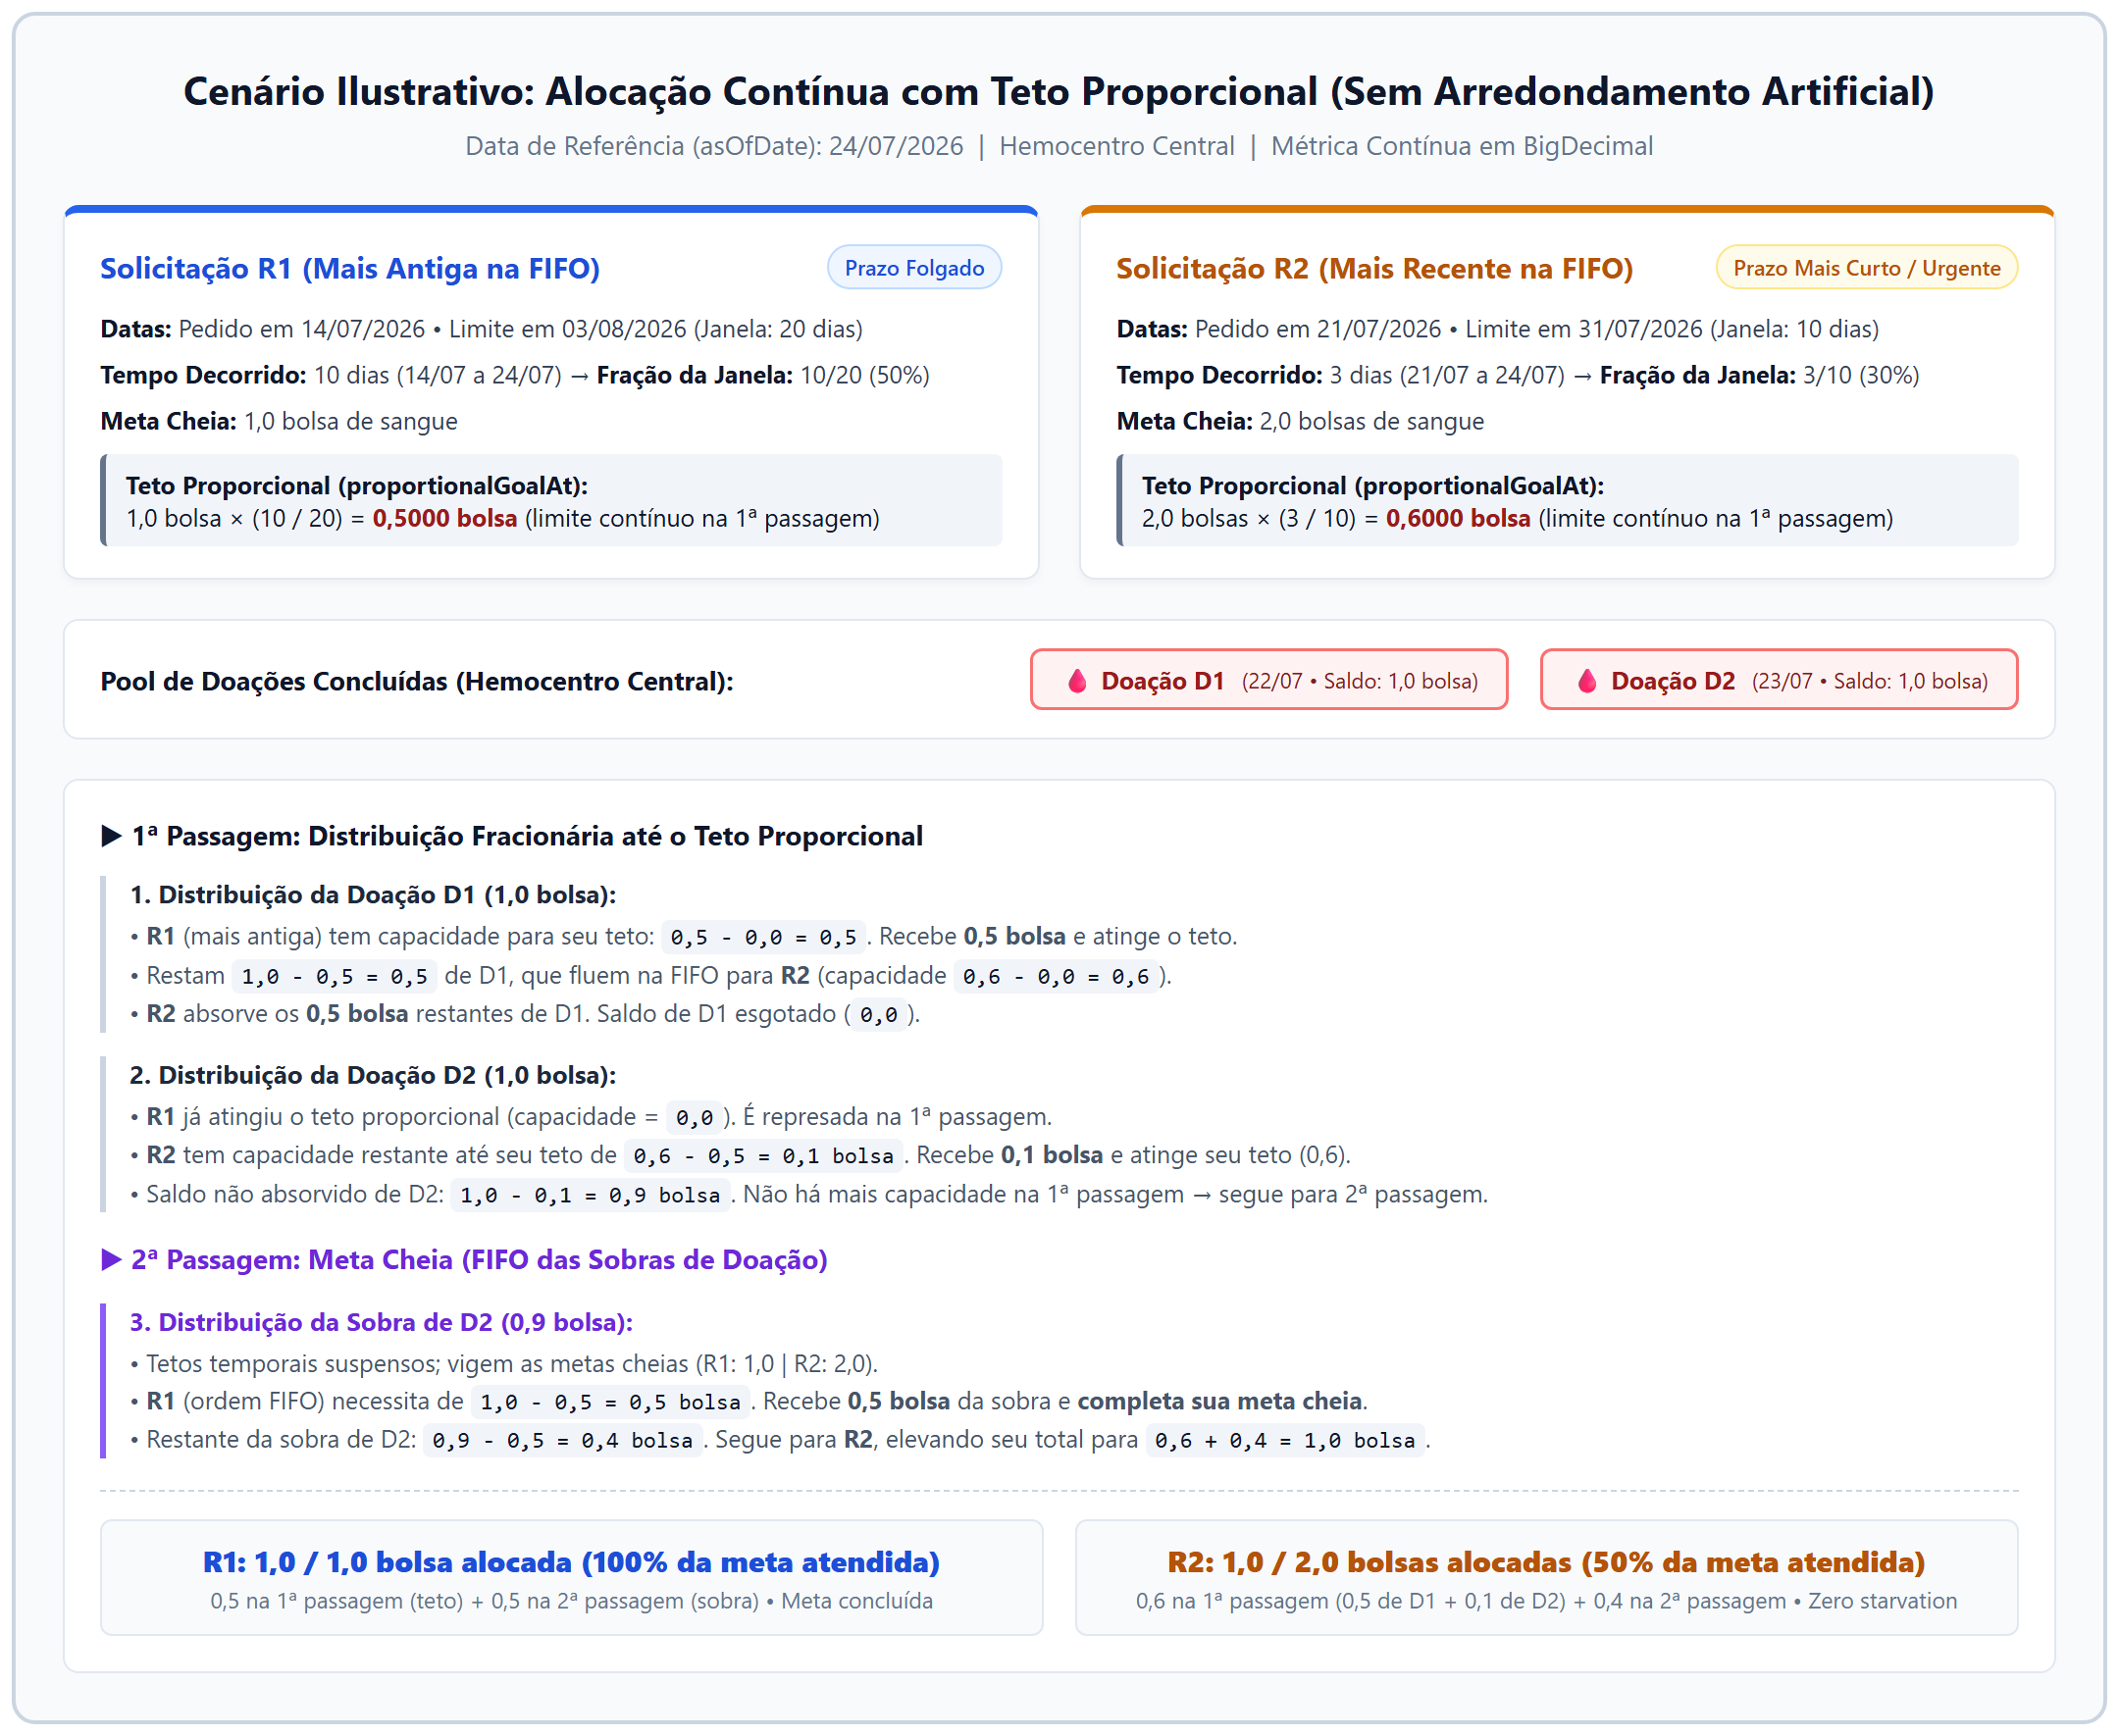
\includegraphics[width=0.98\textwidth]{figura10-exemplo-alocacao-teto}
  \fonte{Elaborado pelos próprios autores (2026).}
  \label{fig:exemplo-alocacao-teto}
\end{figure}

No cenário apresentado, existem duas solicitações ativas concorrendo pelo mesmo \textit{pool} de doações:
\begin{enumerate}[label=\alph*)]
  \item \textbf{Solicitação $R_1$ (mais antiga):} registrada em 14/07 com data-limite em 03/08 (janela total de 20 dias) e meta de 1,0 bolsa. Em 24/07, decorreram 10 dias da janela, correspondendo a uma fração decorrida de $10/20 = 0{,}5$ ($50\%$). Seu teto proporcional calculado é de $1{,}0 \times 0{,}5 = \mathbf{0{,}5000\text{ bolsa}}$;
  \item \textbf{Solicitação $R_2$ (mais recente e mais próxima do limite):} registrada em 21/07 com data-limite em 31/07 (janela total de 10 dias) e meta de 2,0 bolsas. Em 24/07, decorreram 3 dias da janela, correspondendo a uma fração decorrida de $3/10 = 0{,}3$ ($30\%$). Seu teto proporcional calculado é de $2{,}0 \times 0{,}3 = \mathbf{0{,}6000\text{ bolsa}}$.
\end{enumerate}

O hemocentro dispõe de um \textit{pool} com duas doações concluídas compatíveis: $D_1$ (concluída em 22/07, saldo de $1{,}0$ bolsa) e $D_2$ (concluída em 23/07, saldo de $1{,}0$ bolsa). 

Por se tratar de um \textit{snapshot} de alocação dinâmica calculado em memória para mensuração de desempenho puramente matemática --- sem persistência ou associação física estática prévia entre doações e receptores --- o modelo adota a soberania matemática contínua, deixando a distribuição a cargo da matemática sem arredondamentos artificiais:
\begin{itemize}
  \item \textbf{Metas e tetos proporcionais contínuos:} calculados em \codigo{BigDecimal}, permitindo que uma meta liberada temporalmente contenha frações de bolsa (por exemplo, $0{,}5$ ou $1{,}5$ bolsa);
  \item \textbf{Alocação dinâmica contínua:} o quantitativo alocado de uma doação a uma solicitação (\codigo{fulfilledBloodBags}) também pode conter frações de bolsa (por exemplo, $0{,}5$ ou $0{,}7$ bolsa), refletindo com exatidão a parcela da demanda atendida.
\end{itemize}

O fluxo de distribuição em duas passagens opera, portanto, da seguinte forma:
\begin{enumerate}
  \item \textbf{1ª Passagem (Teto Proporcional Contínuo):}
  \begin{itemize}
    \item \textbf{Distribuição de $D_1$ ($1{,}0$ bolsa):} a fila FIFO inicia pela solicitação mais antiga ($R_1$), cuja capacidade restante para atingir o teto é de $0{,}5 - 0{,}0 = 0{,}5$ bolsa. Aloca-se $0{,}5$ bolsa de $D_1$ para $R_1$, que atinge seu teto proporcional ($0{,}5000$). O saldo remanescente de $D_1$ ($1{,}0 - 0{,}5 = 0{,}5$ bolsa) avança na FIFO para $R_2$, que possui capacidade de $0{,}6 - 0{,}0 = 0{,}6$ bolsa. $R_2$ absorve integralmente essa fração restante de $0{,}5$ bolsa, esgotando o saldo de $D_1$ ($0{,}0$);
    \item \textbf{Distribuição de $D_2$ ($1{,}0$ bolsa):} $R_1$ já se encontra no limite do seu teto proporcional (capacidade zero), sendo represada na 1ª passagem. A busca avança para $R_2$, que possui capacidade restante de $0{,}6 - 0{,}5 = 0{,}1$ bolsa. Aloca-se $0{,}1$ bolsa de $D_2$ para $R_2$, que atinge seu teto proporcional ($0{,}6000$). O saldo não absorvido de $D_2$ ($1{,}0 - 0{,}1 = 0{,}9$ bolsa) não encontra mais capacidades disponíveis na 1ª passagem e é encaminhado à 2ª passagem.
  \end{itemize}
  \item \textbf{2ª Passagem (Meta Cheia / FIFO das Sobras):}
  \begin{itemize}
    \item Com os tetos temporais suspensos, aplicam-se as metas cheias ($1{,}0$ para $R_1$ e $2{,}0$ para $R_2$). A sobra de $0{,}9$ bolsa de $D_2$ retorna ao início da fila FIFO;
    \item $R_1$ necessita de $1{,}0 - 0{,}5 = 0{,}5$ bolsa para alcançar sua meta total. Aloca-se $0{,}5$ bolsa da sobra para $R_1$, que conclui integralmente sua meta ($1{,}0/1{,}0$ bolsa, \codigo{goalReached = true});
    \item O restante da sobra ($0{,}9 - 0{,}5 = 0{,}4$ bolsa) avança para $R_2$, elevando seu quantitativo final para $0{,}6 + 0{,}4 = 1{,}0$ bolsa ($50\%$ da meta cheia solicitada).
  \end{itemize}
\end{enumerate}

Ao término do processo, $R_1$ atinge $1{,}0/1{,}0$ bolsa ($100\%$ da meta) e $R_2$ atinge $1{,}0/2{,}0$ bolsas ($50\%$ da meta), com zero desperdício de doações. Nota-se o benefício dessa abordagem matemática: caso o hemocentro dispusesse de apenas uma doação no \textit{pool} ($D_1$ de $1{,}0$ bolsa), a doação seria partilhada exatamente como $0{,}5$ bolsa para $R_1$ e $0{,}5$ bolsa para $R_2$, impedindo que a solicitação mais antiga monopolizasse a única bolsa disponível e permitindo que ambas avançassem proporcionalmente em direção às suas metas.

O progresso (\codigo{fulfilledBloodBags}) não é persistido. Os casos de uso de leitura que precisam exibir o preenchimento --- listagem de solicitações do requisitante, recomendação ao doador e bloqueio de notificação quando a meta já foi atingida --- invocam o mesmo serviço de domínio e recebem o mapa calculado na hora. Concluir uma doação apenas persiste a doação; a leitura seguinte já vê o \textit{pool} atualizado. Como o cálculo não regrava solicitações, não há condição de corrida entre escritas de contador: cada leitura monta o próprio \textit{snapshot}. Assume-se, como contrapartida, que o progresso exibido de uma solicitação de prazo folgado pode decrescer entre duas leituras: à medida que os tetos das solicitações concorrentes crescem com o tempo, bolsas antes atribuídas a ela na segunda passagem migram para solicitações mais próximas do vencimento.

\chapter{Avaliação da proposta de solução}

Este capítulo descreve o plano de avaliação da API desenvolvida, alinhado ao objetivo específico O5 (avaliar a manutenibilidade da solução) e ao objetivo O4 (validar a proposta por meio de estudo de caso e implementação). Como a segunda etapa do trabalho ainda está em andamento, as seções a seguir apresentam o que será avaliado e como, e não os resultados finais, que serão consolidados na versão definitiva desta monografia.

\section{Plano de avaliação}

A avaliação da solução será conduzida em duas frentes complementares. A primeira, de caráter funcional, apoia-se em testes automatizados: testes unitários para as regras de negócio isoladas no domínio (por exemplo, elegibilidade do doador, compatibilidade sanguínea e a alocação FIFO do \texttt{DonationRequestFulfillmentService}) e testes de integração para os fluxos que atravessam as camadas de aplicação, persistência e segurança (como a criação de uma solicitação seguida de doações concluídas e a consequente atualização de \texttt{fulfilledBloodBags}). A segunda frente, de caráter estrutural, avalia a manutenibilidade da API à luz dos princípios SOLID e do DDD apresentados no Capítulo~2, verificando se a separação em camadas (\texttt{domain}, \texttt{application/usecase}, \texttt{interfaces/rest}, \texttt{infra/persistence} e \texttt{infra/security}) de fato isola as regras de negócio de detalhes de infraestrutura, conforme descrito no Capítulo~5.

\section{Resultados}

Esta seção apresentará, na versão final do trabalho, a cobertura e os resultados obtidos com a suíte de testes unitários e de integração, bem como eventuais evidências qualitativas de manutenibilidade (como a facilidade de estender um novo caso de uso ou de substituir uma implementação de infraestrutura sem alterar o domínio). No momento da entrega desta versão, a implementação da API e a suíte de testes correspondente ainda estão em desenvolvimento, de modo que os resultados quantitativos não são apresentados aqui.

\section{Sugestões de melhorias}

A partir dos resultados da avaliação, esta seção reunirá melhorias identificadas ao longo da validação --- por exemplo, ajustes no algoritmo de alocação de doações, na cobertura de testes de casos de borda (solicitações expiradas, doações concorrentes) ou na experiência de consumo da API evidenciada pela documentação OpenAPI. Como a avaliação ainda não foi concluída, este trabalho não antecipa melhorias específicas nesta versão.

\section{Considerações sobre a avaliação}

Ao final da avaliação, esta seção sintetizará em que medida a API construída atendeu aos objetivos O3, O4 e O5, discutindo a eficácia da estratégia de recomendação e de cumprimento de metas descrita no Capítulo~5 e o grau de manutenibilidade alcançado pela arquitetura em camadas orientada a DDD. Essa síntese será redigida somente após a execução do plano de avaliação descrito neste capítulo.

\chapter{Considerações finais}

Este capítulo retoma a problemática apresentada na Introdução à luz do sistema desenvolvido (Capítulo~5) e dos resultados da avaliação (Capítulo~6), discutindo o alcance dos objetivos, as principais contribuições do trabalho e direcionamentos para pesquisas e evoluções futuras.

\section{Alcance dos objetivos}

O objetivo geral --- gerenciar as doações de sangue a partir de um sistema de informações via Web, aproximando solicitações de unidades de saúde e pacientes dos doadores compatíveis --- foi alcançado por meio da implementação descrita no Capítulo~5. A verificação automatizada relatada no Capítulo~6 constitui o passo metodológico de avaliação da proposta, e não uma entrega autônoma.

No que tange aos objetivos específicos estabelecidos, constata-se que todos foram plenamente atendidos no escopo do trabalho. O primeiro objetivo específico (O1) concretizou-se por meio do mapeamento aprofundado dos processos hemoterápicos, culminando na modelagem da hierarquia de participantes (\codigo{Party}, \codigo{Person} e \codigo{Organization}), na definição dinâmica de seus papéis (\codigo{Donor}, \codigo{Requester} e \codigo{BloodCenter}) e na estruturação dos agregados centrais \codigo{DonationRequest} e \codigo{Donation}, detalhados no Capítulo~5.

O segundo objetivo específico (O2) foi alcançado com a condução do mapeamento sistemático da literatura apresentado no Capítulo~3, o qual possibilitou identificar o estado da arte e as lacunas nos sistemas existentes, fornecendo subsídios teóricos e práticos que nortearam as decisões de projeto para recomendação, notificação ativa e gestão de demandas. Por sua vez, o terceiro objetivo específico (O3) materializou-se na concepção e codificação dos serviços de matching e recomendação geoespacial compatível e na notificação dirigida a voluntários elegíveis --- por meio de casos de uso como \codigo{GetRecommendedRequestsUseCase}, \codigo{FindEligibleDonorsUseCase}, \codigo{DonorMatchingService} e \codigo{NotifyPotentialDonorsUseCase} ---, sendo a eficácia e a corretude de tais componentes formalmente corroboradas pela execução da suíte de testes automatizados apresentada no Capítulo~6. Desse modo, evidencia-se o atendimento harmônico e integral dos objetivos propostos para a pesquisa.

\section{Principais contribuições}

Do ponto de vista acadêmico, este trabalho oferece contribuições ao sistematizar o conhecimento sobre sistemas de captação de doadores por meio de um mapeamento sistemático da literatura, ao formalizar um estudo de caso de engenharia de \textit{software} aplicando DDD e princípios SOLID a um domínio crítico de saúde pública com restrições biológicas e temporais, e ao fornecer uma metodologia explícita de avaliação estruturada em suíte de testes automatizados que torna verificáveis as regras de negócio essenciais.

No plano tecnológico, a principal contribuição consolida-se no desenvolvimento da API RESTful \textit{BloodMatch}. Destaca-se a concepção da estratégia de recomendação personalizada que combina proximidade e critérios clínicos, bem como o algoritmo de cumprimento de metas calculado por \textit{snapshot} em memória. Esse algoritmo introduz uma abordagem de racionamento em que a alocação FIFO de bolsas é modulada por um teto proporcional ao tempo de vigência da solicitação, repartindo a escassez em favor das demandas mais urgentes e prevenindo concorrência em contadores persistidos. A solução é complementada por um modelo seguro de autenticação e autorização via JWT com validação de posse (\textit{ownership}) dos recursos e por uma arquitetura em camadas desacopladas que preserva a pureza do domínio em relação a protocolos de transporte e esquemas de armazenamento, servindo de base arquitetural para aplicações correlatas na área da saúde.

\section{Limitações}

Apesar dos resultados positivos, reconhecem-se limitações. A avaliação funcional privilegiou testes unitários e de integração com \textit{mocks}, sem mensuração sistemática de cobertura percentual de linhas/branches nem baterias de carga em produção. O \textit{snapshot} de preenchimento relê o pool do hemocentro a cada consulta que exibe progresso, o que privilegia simplicidade e consistência em detrimento de um contador materializado. Como consequência do teto proporcional sobre esse recálculo, o progresso exibido de uma solicitação de prazo folgado pode decrescer entre duas leituras, quando bolsas migram para solicitações mais próximas do vencimento --- comportamento correto do ponto de vista da política de racionamento, mas cuja apresentação ao requisitante merece tratamento específico na interface. Além disso, o estudo de caso não inclui avaliação formal de usabilidade com usuários finais de hemocentros.

\section{Trabalhos futuros}

Como direcionamentos para trabalhos e pesquisas futuras, vislumbra-se aprimorar o algoritmo de recomendação com a introdução de critérios heurísticos e comportamentais adicionais, tais como a taxa de resposta histórica dos voluntários e padrões sazonais de doação. Do ponto de vista arquitetural, sugere-se evoluir o particionamento do sistema mediante a extração de módulos Maven ou microsserviços independentes para os contextos delimitados do DDD, reforçando os limites transacionais hoje estabelecidos por convenção de pacotes.

Sob a perspectiva da engenharia de testes, recomenda-se a expansão da suíte por meio da adoção de contêineres gerenciados para testes com banco real, da geração automatizada de relatórios de cobertura de código e da execução sistemática de testes de carga e de contrato da API. Por fim, no plano aplicado, mostra-se fundamental conduzir estudos empíricos integrados ao cotidiano operacional de hemocentros reais, permitindo avaliar a usabilidade e quantificar o impacto efetivo da plataforma na conversão de solicitações em doações realizadas.

\section{Considerações finais}

O descompasso entre demanda e oferta de sangue, contextualizado na Introdução, motiva soluções tecnológicas que aproximem requisitantes e doadores com critérios clinicamente relevantes --- tipagem, elegibilidade e proximidade ---, convergindo com as metas de acesso a serviços essenciais de saúde preconizadas pelo ODS~3 da ONU. Este trabalho respondeu a essa necessidade com uma API RESTful orientada ao domínio da doação sanguínea, validada por implementação e por 156 testes automatizados sem falhas.

Conclui-se que a combinação de DDD, SOLID e testes automatizados favoreceu não apenas a entrega funcional dos requisitos, mas também a confiança na corretude das regras críticas e a perspectiva de manutenção evolutiva da solução. Espera-se que os artefatos e os resultados aqui apresentados subsidiem trabalhos futuros e inspirem aprimoramentos em sistemas de apoio à captação de doadores de sangue.


% ============================================================================
% ELEMENTOS PÓS-TEXTUAIS
% ============================================================================
\postextual

\printbibliography

% ============================================================================
% APÊNDICES (NBR 14724: material elaborado pelo autor)
% ============================================================================
\begin{apendicesenv}
% !TeX root = ../main.tex
\chapter{Regras de domínio: tipagem sanguínea e elegibilidade}
\label{ap:regras-dominio}

Este apêndice apresenta trechos do código-fonte que materializam regras centrais do domínio da doação sanguínea: a compatibilidade tipológica, encapsulada no objeto de valor \codigo{BloodType}, e a elegibilidade temporal do doador, encapsulada na entidade \codigo{Donor}. Ambos os trechos pertencem à camada \codigo{domain} e não dependem de infraestrutura.

\section{Compatibilidade tipológica}

A Listagem~\ref{lst:bloodtype-candonateto} reproduz o método \codigo{canDonateTo} do objeto de valor \codigo{BloodType}. A regra é expressa por um \textit{switch} sobre o tipo do doador, retornando \texttt{true} somente quando o receptor é clinicamente compatível. O caso \texttt{O-} doa para qualquer tipo; o caso \texttt{AB+} doa apenas para \texttt{AB+}.

\lstinputlisting[
  language=Java,
  caption={Método \texttt{BloodType.canDonateTo}},
  label={lst:bloodtype-candonateto}
]{apendices/codigo/BloodTypeCanDonateTo.java}
\fonte{Elaborado pelos próprios autores (2026).}

\section{Elegibilidade do doador}

A Listagem~\ref{lst:donor-eligible} apresenta a verificação de elegibilidade: faixa etária entre 16 e 69~anos e intervalo mínimo desde a última doação, definido por \codigo{DonationPolicy}. Se não houver doação prévia, o doador é considerado elegível do ponto de vista temporal.

\lstinputlisting[
  language=Java,
  caption={Métodos \texttt{Donor.hasValidAge} e \texttt{Donor.isEligibleToDonate}},
  label={lst:donor-eligible}
]{apendices/codigo/DonorIsEligibleToDonate.java}
\fonte{Elaborado pelos próprios autores (2026).}

% !TeX root = ../main.tex
\chapter{Agregados: aceitação de doação e ciclo de vida}
\label{ap:agregados}

Este apêndice reúne trechos das raízes de agregado \codigo{DonationRequest} e \codigo{Donation}, evidenciando a proteção de invariantes no núcleo do domínio --- princípio tático do DDD discutido no Capítulo~2 e materializado na modelagem do Capítulo~5.

\section{Aceitação de doação pela solicitação}

A Listagem~\ref{lst:accepts-donation} mostra o método \codigo{acceptsDonation}, usado pelo algoritmo de cumprimento de metas (Apêndice~\ref{ap:fulfillment}). A solicitação só aceita a doação se estiver ativa, não expirada, se a doação estiver concluída, se a data da doação estiver na janela \texttt{[dateRequested, dateLimit]} e se o tipo sanguíneo do doador for compatível com o tipo solicitado.

\lstinputlisting[
  language=Java,
  caption={Método \texttt{DonationRequest.acceptsDonation}},
  label={lst:accepts-donation}
]{apendices/codigo/DonationRequestAcceptsDonation.java}
\fonte{Elaborado pelos próprios autores (2026).}

\section{Conclusão de doação pendente}

A Listagem~\ref{lst:donation-complete} ilustra a máquina de estados da doação: \codigo{validateStatusFlags} exige exatamente um estado ativo entre pendente, concluída e cancelada; \codigo{complete} só permite a transição a partir de pendente e rejeita datas futuras.

\lstinputlisting[
  language=Java,
  caption={Validação de estado e método \texttt{Donation.complete}},
  label={lst:donation-complete}
]{apendices/codigo/DonationComplete.java}
\fonte{Elaborado pelos próprios autores (2026).}

% !TeX root = ../main.tex
\chapter{Cumprimento de metas FIFO e matching de doadores}
\label{ap:fulfillment}

Este apêndice documenta o núcleo algorítmico da solução: a alocação \textit{First In, First Out} (FIFO) de doações concluídas às solicitações ativas de um hemocentro e o serviço de domínio que identifica doadores elegíveis para notificação.

\section{Alocação FIFO de doações}

A Listagem~\ref{lst:fifo} sintetiza o caminho de leitura do \codigo{DonationRequestFulfillmentService}: \codigo{fill} recebe o hemocentro e a data de referência \codigo{asOfDate}, carrega somente as solicitações ativas e não expiradas daquele centro, e \codigo{allocateLoaded} busca as doações concluídas na janela \codigo{[pedido ativo mais antigo, asOfDate]}. Em seguida, \codigo{allocateFifo} isola o pool por hemocentro, ordena solicitações e doações da mais antiga para a mais nova e atribui cada doação à primeira solicitação que ainda cabe na meta e que \codigo{acceptsDonation} aceita --- o \texttt{break} encerra a busca, concretizando a política FIFO. O resultado permanece em memória: nada é persistido.

\lstinputlisting[
  language=Java,
  caption={Alocação FIFO em \texttt{DonationRequestFulfillmentService}},
  label={lst:fifo}
]{apendices/codigo/FulfillmentDistributeDonations.java}
\fonte{Elaborado pelos próprios autores (2026).}

\section{Identificação de doadores elegíveis}

A Listagem~\ref{lst:matching} apresenta \codigo{DonorMatchingService.findEligibleDonors}, que compõe compatibilidade tipológica (\codigo{canBeFulfilledBy}), elegibilidade temporal (\codigo{isEligibleToDonate}) e proximidade geográfica limitada pela distância máxima configurada pelo doador.

\lstinputlisting[
  language=Java,
  caption={Método \texttt{DonorMatchingService.findEligibleDonors}},
  label={lst:matching}
]{apendices/codigo/DonorMatchingService.java}
\fonte{Elaborado pelos próprios autores (2026).}

% !TeX root = ../main.tex
\chapter{Inversão de dependência: repositório e caso de uso}
\label{ap:dip}

Este apêndice exemplifica a aplicação do princípio da inversão de dependência (SOLID) na arquitetura da API: o caso de uso depende de abstrações de repositório definidas no domínio, e não de implementações concretas de persistência.

\section{Contrato de repositório}

A Listagem~\ref{lst:donation-repo} apresenta a interface \codigo{DonationRepositoryInterface}, situada na camada \codigo{domain}. Operações de leitura e escrita são expressas em termos do agregado \codigo{Donation} e do objeto de valor \codigo{DomainID}, sem menção a MongoDB ou a \textit{schemas} de persistência.

\lstinputlisting[
  language=Java,
  caption={Interface \texttt{DonationRepositoryInterface}},
  label={lst:donation-repo}
]{apendices/codigo/DonationRepositoryInterface.java}
\fonte{Elaborado pelos próprios autores (2026).}

\section{Orquestração no caso de uso}

A Listagem~\ref{lst:complete-pending} mostra o método \codigo{execute} de \codigo{CompletePendingDonationUseCase}. O fluxo valida a entrada, carrega a doação via repositório, verifica \textit{ownership}, delega a transição de estado ao agregado (\codigo{donation.complete}), atualiza o doador e persiste a doação concluída. O cumprimento de metas não é gravado nesse momento: a leitura seguinte monta o \textit{snapshot} FIFO a partir do banco.

\lstinputlisting[
  language=Java,
  caption={Método \texttt{CompletePendingDonationUseCase.execute}},
  label={lst:complete-pending}
]{apendices/codigo/CompletePendingDonationUseCase.java}
\fonte{Elaborado pelos próprios autores (2026).}

\end{apendicesenv}

\end{document}
